\documentclass[12pt,letterpaper,oneside]{report}
\usepackage[utf8]{inputenc}
\usepackage[T1]{fontenc}
\usepackage[spanish,es-tabla]{babel}
\usepackage{mathptmx}
\usepackage[scaled=0.92]{helvet}
\usepackage[letterpaper,left=2.5cm,right=2.5cm,top=2.5cm,bottom=2.5cm,footskip=1.0cm]{geometry}
\usepackage{setspace}
\usepackage{amsmath,amssymb,amsfonts}
\usepackage{graphicx}
\usepackage{textcomp}
\usepackage{booktabs}
\usepackage{multirow}
\usepackage{url}
\usepackage{cite}
\usepackage{titlesec}
\usepackage{fancyhdr}
\usepackage[font={small},labelfont=bf,justification=raggedright,singlelinecheck=false]{caption}
\usepackage{tocloft}
\usepackage[hidelinks]{hyperref}

% Guia UNAB: interlineado 1,5; texto justificado; titulos a la izquierda en mayusculas y negrita
\onehalfspacing
\setlength{\parindent}{0pt}
\setlength{\parskip}{0.6\baselineskip}
\addto\captionsspanish{\renewcommand{\contentsname}{TABLA DE CONTENIDOS}\renewcommand{\listfigurename}{ÍNDICE DE FIGURAS}\renewcommand{\listtablename}{ÍNDICE DE TABLAS}\renewcommand{\bibname}{REFERENCIAS BIBLIOGRÁFICAS}}
\titleformat{\chapter}[block]{\normalfont\large\bfseries}{\thechapter}{0.8em}{}
\titlespacing*{\chapter}{0pt}{0pt}{24pt}
\titleformat{\section}[block]{\normalfont\bfseries}{\thesection}{0.6em}{}
\titleformat{\subsection}[block]{\normalfont\bfseries\itshape}{\thesubsection}{0.6em}{}
\titleformat{\chapter}[block]{\normalfont\large\bfseries}{\thechapter}{0.8em}{}
\renewcommand{\cftchapfont}{\bfseries}
\renewcommand{\cftchappagefont}{\bfseries}
\setlength{\cftbeforechapskip}{4pt}

% Numeracion de pagina: esquina inferior derecha, sin la palabra "pagina"
\pagestyle{fancy}\fancyhf{}\renewcommand{\headrulewidth}{0pt}\fancyfoot[R]{\thepage}
\fancypagestyle{plain}{\fancyhf{}\renewcommand{\headrulewidth}{0pt}\fancyfoot[R]{\thepage}}
\fancypagestyle{portada}{\fancyhf{}\renewcommand{\headrulewidth}{0pt}}

\begin{document}
\pagenumbering{roman}

% ---------------- PORTADA (formato general UNAB: una pagina completa; se cuenta pero no se numera) ----------------
\thispagestyle{portada}
\begin{singlespace}
\begin{center}
\vspace*{0.3cm}

\includegraphics[height=4.2cm]{logo_unab_portada.png}\\[1.2cm]
{\rmfamily\bfseries\large UNIVERSIDAD ANDRÉS BELLO}\\[0.5cm]
{\rmfamily\bfseries\large FACULTAD DE INGENIERÍA}\\[1.2cm]
{\rmfamily\bfseries\large INGENIERÍA CIVIL INFORMÁTICA}\\[1.6cm]
{\sffamily\bfseries\large\underline{Modelo Predictivo de Resultados de Partidos de la Premier League (2017/2025)}}\\[3.0cm]
{\sffamily\bfseries\large ANAKIN ADOLFO BENAVIDES ROMERO}\\[0.2cm]
{\sffamily\bfseries\large SEBASTIÁN IGNACIO VALDOVINOS BRAVO}\\[0.5cm]
{\rmfamily\bfseries\large Profesor guía: Pablo Hernán Schwarzenberg Riveros}\\
\vfill
{\sffamily\bfseries\large SANTIAGO -- CHILE}\\[0.4cm]
{\sffamily\bfseries\large Noviembre, 2026}
\vspace*{0.5cm}
\end{center}
\end{singlespace}
\clearpage

% ---------------- DECLARACION DE ORIGINALIDAD ----------------
\begin{center}{\bfseries\underline{DECLARACIÓN DE AUTORÍA Y ORIGINALIDAD DEL TRABAJO DE TITULACIÓN}}\end{center}
\vspace{1cm}
En relación con el trabajo de titulación presentado para su defensa y evaluación, se declara la originalidad del mismo, entendiéndose que no se han utilizado fuentes sin citarlas debidamente.

\vspace{3cm}
\begin{center}
\begin{tabular}{@{}p{6.5cm}p{6.5cm}@{}}
\rule{6cm}{0.4pt} & \rule{6cm}{0.4pt}\\
Anakin Adolfo Benavides Romero & Sebastián Ignacio Valdovinos Bravo
\end{tabular}
\end{center}
\vspace{2cm}
\begin{center}Santiago, Chile, noviembre de 2026\end{center}
\clearpage

% ---------------- TABLA DE CONTENIDOS E INDICES ----------------
\tableofcontents
\clearpage
\listoffigures
\clearpage
\listoftables
\clearpage

% ---------------- RESUMEN Y ABSTRACT ----------------
\chapter*{RESUMEN}
\addcontentsline{toc}{chapter}{RESUMEN}
\begin{singlespace}
Este proyecto compara modelos de aprendizaje de máquinas para predecir si el equipo local gana un partido de la Premier League (victoria local o no victoria local), con datos de las temporadas 2017/2018 a 2024/2025. Se construyó un conjunto de datos con estadísticas de partidos, planteles y cuotas de apuestas, del que se derivaron variables de forma reciente, enfrentamientos directos, calidad del plantel y rendimiento de porteros. Se evaluaron siete modelos, incluida una red neuronal optimizada con Keras Tuner, con validación temporal de ventana expansiva (7 folds). Un control de calidad detectó y corrigió dos errores en los datos (partidos duplicados con cuotas de otro partido y fechas con día y mes invertidos) que dejaban partidos futuros dentro de la forma reciente e inflaban las métricas: con los datos corregidos el mejor modelo de la comparación principal, Random Forest, alcanza 68,2\% de accuracy y ROC-AUC de 0,727 (antes 74,2\% y 0,806). Ese resultado supera en 3,9 puntos porcentuales a la regla simple del mercado de apuestas (64,4\%) en los 7 folds, pero ningún modelo supera a una regresión logística entrenada solo con las probabilidades de las cuotas (68,6\%). Las variables de forma, plantel y una mezcla de modelos no aportan mejoras medibles, y sin cuotas los modelos solo igualan a la regla simple. Una prueba con la temporada 2025/26, no usada en el desarrollo, dio 61,3\% (Random Forest) y 62,9\% (solo cuotas) frente a 60,5\% del mercado, sin diferencias significativas, y un análisis de error por equipo mostró que los errores se concentran en partidos parejos y empates y son en su mayoría compartidos con el mercado. Se concluye que las cuotas concentran la mayor parte de la información predecible, en línea con la literatura.
\end{singlespace}

\textbf{Palabras clave:} aprendizaje de máquinas, calidad de datos, fuga de información, interpretabilidad SHAP, Keras Tuner, mercado de apuestas, predicción de fútbol, Premier League, validación temporal.

\clearpage
\chapter*{ABSTRACT}
\addcontentsline{toc}{chapter}{ABSTRACT}
\begin{singlespace}
This project compares machine learning models to predict whether the home team wins a Premier League match (home win vs.\ no home win), using data from the 2017/2018 to 2024/2025 seasons. A dataset was built with match statistics, squads and betting odds, from which recent-form, head-to-head, squad-quality and goalkeeper-performance variables were derived. Seven models were evaluated, including a neural network tuned with Keras Tuner, using expanding-window temporal validation (7 folds). A quality-control process detected and corrected two data errors (duplicated matches carrying the odds of another match, and dates with day and month swapped) that left future matches inside the recent-form windows and inflated the metrics: with the corrected data, the best model of the main comparison, Random Forest, reaches 68.2\% accuracy and a ROC-AUC of 0.727 (previously 74.2\% and 0.806). This result exceeds the simple betting-market rule (64.4\%) by 3.9 percentage points in all 7 folds, but no model outperforms a logistic regression trained only on the probabilities implied by the odds (68.6\%). Form and squad variables and a blend of models provide no measurable improvement, and without odds the models only match the simple rule. A test on the 2025/26 season, not used during development, gave 61.3\% (Random Forest) and 62.9\% (odds only) against 60.5\% for the market, with no significant differences, and an error analysis by team showed that errors concentrate in evenly matched games and draws and are mostly shared with the market. It is concluded that the odds concentrate most of the predictable information, in line with the literature.
\end{singlespace}

\textbf{Keywords:} machine learning, data quality, data leakage, SHAP interpretability, Keras Tuner, betting market, football prediction, Premier League, temporal validation.

\clearpage
\pagenumbering{arabic}

\chapter{INTRODUCCIÓN}
\label{sec:introduction}
La predicción de resultados deportivos ha experimentado un crecimiento exponencial en la última década, impulsado por la disponibilidad masiva de datos estadísticos y el avance de las técnicas de aprendizaje de máquinas (\textit{machine learning}). En particular, el fútbol de élite ---y la Premier League inglesa como su exponente más popular a nivel mundial--- genera millones de datos por temporada: estadísticas de partidos, métricas individuales de jugadores, datos de rendimiento físico y señales del mercado de apuestas, entre otros.

En este contexto, el presente proyecto de título tiene como propósito central desarrollar un modelo predictivo capaz de anticipar el resultado de partidos de la Premier League, utilizando técnicas supervisadas de aprendizaje de máquinas y un conjunto de datos histórico construido especialmente para este fin. El período de análisis abarca ocho temporadas completas (2017/2018 a 2024/2025).

La motivación radica en la brecha entre los sistemas de predicción de la literatura ---mayoritariamente basados en estadísticas básicas como goles y puntos acumulados--- y la riqueza de datos contextuales disponibles hoy: forma reciente, características del plantel, rendimiento de los porteros y señales implícitas del mercado de apuestas. La hipótesis de trabajo fue que incorporar estas variables mejora la capacidad predictiva respecto de enfoques clásicos y del mercado de apuestas como \textit{benchmark}. Esa hipótesis se contrasta con validación temporal estricta y con un control explícito de la calidad de los datos.

El trabajo se estructura así: contexto del problema (Capítulo~\ref{sec:contexto}), objetivos (Capítulo~\ref{sec:objetivos}), estado del arte (Capítulo~\ref{sec:estado}), ingeniería del proyecto (Capítulo~\ref{sec:ingenieria}), resultados (Capítulo~\ref{sec:resultados}), discusión y limitaciones (Capítulo~\ref{sec:discusion}) y conclusiones (Capítulo~\ref{sec:conclusiones}).

\chapter{CONTEXTO DEL PROBLEMA}
\label{sec:contexto}

\section{La Premier League como objeto de estudio}
La Premier League es una de las ligas de fútbol profesional más seguidas del mundo. Cada temporada se disputan 380 partidos entre 20 clubes, lo que genera un volumen considerable de datos estadísticos, económicos y deportivos. Su alta competitividad incrementa la incertidumbre de los resultados y genera una tasa natural de resultados impredecibles que ningún modelo puede eliminar por completo.

\section{Complejidad del problema de predicción}
Predecir el resultado de un partido es un problema de clasificación binaria (victoria local vs. no victoria local) con tres características particulares:
\begin{itemize}
\item \textbf{Alta variabilidad intrínseca:} incluso entre equipos de calidad similar, el resultado depende de factores difícilmente cuantificables, como el estado físico de jugadores clave, las condiciones climatológicas o las decisiones tácticas.
\item \textbf{Distribución de clases desequilibrada:} en el conjunto de datos de este proyecto el local gana el 44,2\% de los partidos, lo que dificulta predecir correctamente las victorias visitantes.
\item \textbf{Dependencia temporal:} el rendimiento de los equipos evoluciona durante la temporada; un modelo que no respete el orden cronológico incurre en \textit{data leakage} y sobreestima su desempeño real.
\end{itemize}
La variable objetivo (\texttt{target\_home\_win}) es binaria: vale 1 si el equipo local gana y 0 en caso contrario.

\section{Relevancia del mercado de apuestas como benchmark}
Las cuotas de las casas de apuestas resumen la información pública disponible sobre cada partido y son un referente exigente: tanto Baboota y Kaur~\cite{baboota2019predictive} como Ridall et al.~\cite{ridall2025bayesian} reportan que sus modelos no superaron a las casas de apuestas medido con RPS. En este proyecto se usan dos referencias del mercado. La primera es una \textit{regla simple}: predecir victoria local cuando la probabilidad implícita de la cuota del local supera a la del visitante, que alcanza un accuracy de 64,4\% en las siete temporadas de evaluación (64,3\% con las ocho). La segunda es más exigente: una regresión logística entrenada, con la misma validación temporal, solo con las tres probabilidades implícitas de las cuotas (local, empate y visitante). La literatura reporta accuracies de 50 a 78\% para predicción de resultados~\cite{ricogonzalez2023ml}.

\section{Pregunta de investigación e hipótesis}
\label{sec:pregunta}
¿Es posible predecir con mayor exactitud que el mercado de apuestas si el equipo local gana un partido de la Premier League, utilizando únicamente información pública disponible antes del partido y una validación temporal que impida el uso de datos futuros?

Como hipótesis de trabajo se planteó que un modelo que incorpora forma reciente, enfrentamientos directos, calidad del plantel, rendimiento de porteros y cuotas predice mejor que la regla simple del mercado (apostar por el favorito de las cuotas) y que un modelo entrenado solo con las cuotas. Ambas comparaciones se contrastan en el Capítulo~
ef{sec:resultados}.

\chapter{OBJETIVOS DEL PROYECTO}
\label{sec:objetivos}

\section{Objetivo general}
Desarrollar un modelo de aprendizaje de máquinas capaz de predecir el resultado (victoria local o no victoria local) de partidos de la Premier League, a partir de datos históricos de las temporadas 2017/2018 a 2024/2025, superando el desempeño del mercado de apuestas como referencia de comparación.

\section{Objetivos específicos}
\begin{enumerate}
\item Recolectar, limpiar y consolidar datos históricos de partidos desde la temporada 2017/2018 a 2024/2025, incluyendo estadísticas de rendimiento, calidad de planteles y cuotas del mercado de apuestas, y validar su calidad.
\item Diseñar e implementar un proceso de \textit{feature engineering} que capture la forma reciente de los equipos (ventana móvil de 5 partidos), el historial de enfrentamientos directos, la calidad del plantel y el rendimiento de porteros.
\item Entrenar y comparar algoritmos de clasificación supervisada (Gradient Boosting, Random Forest, Regresión Logística, SVM RBF, MLP y redes neuronales en PyTorch y en Keras con Keras Tuner) con validación temporal y optimización de hiperparámetros.
\item Evaluar el desempeño con accuracy, F1-Score, ROC-AUC, Brier Score y log-loss, y compararlo con el \textit{baseline} del mercado.
\item Aplicar análisis de interpretabilidad (importancia Gini, de permutación y valores SHAP) para identificar los factores más relevantes de la predicción.
\item Documentar el proceso completo en un informe académico formal.
\end{enumerate}

\chapter{ESTADO DEL ARTE}
\label{sec:estado}

\section{Panorama general de la predicción en fútbol}
Los primeros trabajos ---predominantes en la década de 2000--- usaban modelos estadísticos clásicos como la regresión de Poisson y los modelos de Dixon-Coles para estimar la distribución de goles. Desde 2015, el acceso a datos más ricos y el desarrollo de algoritmos de \textit{ensemble learning} provocaron un giro hacia enfoques de \textit{machine learning}, con Gradient Boosting y Random Forest como los métodos más reportados~\cite{ricogonzalez2023ml}. La revisión identifica dos paradigmas: la clasificación directa del resultado mediante ML supervisado, y el enfoque probabilístico-estadístico basado en modelos de conteo de goles y sistemas dinámicos de estado.

\section{Trabajos analizados}
La Tabla~\ref{tab:literatura} resume los diez trabajos revisados.

\begin{table}[!htbp]
\caption[Comparación de trabajos revisados: liga, dataset, resultado y aporte principal]{Comparación de trabajos revisados: liga, dataset, resultado y aporte principal.}
\label{tab:literatura}
\setlength{\tabcolsep}{2pt}
\footnotesize
\begin{tabular}{@{}p{3.2cm}p{2.2cm}p{3.4cm}p{2.6cm}p{4.6cm}@{}}
\toprule
\textbf{Referencia} & \textbf{Liga} & \textbf{Dataset} & \textbf{Mejor resultado} & \textbf{Limitación / aporte} \\
\midrule
Vujčić et al. (2026)~\cite{vujcic2026supervised} & EPL (fbref.com) & 2.292 registros equipo-partido; corte 1-ene-2022 & RF: 77,01\% (promedio por equipo) & 7 algoritmos; modelos por equipo; un único corte temporal \\
Ajulo y Tiamiyu (2026)~\cite{ajulo2026ml} & EPL 2021--2025 & 5 temporadas, football-data.co.uk; 3 clases & RF: 87,14\%; AUC 99\% & Partición temporal 70/15/15; variables del propio partido (posible fuga) \\
Ravichandran y Sani (2026)~\cite{ravichandran2026framework} & EPL, éxito de equipo por temporada & Kaggle, jugadores 1992--2019 & GB; F1 $\approx$ 1,00 & Estudio piloto (preprint); no predice partidos; SHAP \\
Chowdary (2026)~\cite{chowdary2026dynamic} & IPL (cricket) + EPL & IPL 2018--2024 (457); EPL 2001--2025 (9.380) & IPL: 54,3\% $>$ Elo ($p=0{,}003$); EPL: 67,7\% $\approx$ Elo & Matrices de probabilidad relativa; preprint \\
Ridall et al. (2025)~\cite{ridall2025bayesian} & EPL 1992--2024 & Entrena 1992/93--2009/10; test 2010/11--2023/24 & RPS acum. 17,55 & Bayesiano estado-espacio; ninguno superó a las cuotas \\
Howell et al. (2026)~\cite{howell2026winning} & Premier League 2 & 367 partidos (303 train, 64 test), Wyscout & Reg. log.: 58,3\%; AUC 0,771 (test) & KPIs en liga de reservas \\
Sjöberg (2023)~\cite{sjoborg2023football} & Bundesliga 2015--16 & 219 partidos útiles (de 306); atributos FIFA & Reg. log.: 63,0\% (3 clases) & Bajo volumen; partición aleatoria 70/30 \\
Rico-González et al. (2023)~\cite{ricogonzalez2023ml} & Revisión sistemática & 32 estudios & RF, DT, KNN: 50--78\% & Baja reproducibilidad \\
Li y Hong (2022)~\cite{li2022football} & Fútbol (liga no especificada) & Test de 10 partidos & Red BP: 80\% (KNN 40\%, LR 60\%) & Edge computing; muestra de test mínima \\
Baboota y Kaur (2019)~\cite{baboota2019predictive} & EPL & 2005--2016; test 2014--2016; 3 clases & GB: RPS 0,2156 (cuotas: 0,2012) & Ratings FIFA; sin porteros; no superó a las cuotas \\
\bottomrule
\end{tabular}
\par\smallskip{\footnotesize Fuente: elaboración propia a partir de las referencias citadas.}
\end{table}

\textbf{Vujčić et al.}~\cite{vujcic2026supervised} es el trabajo más comparable en liga y algoritmos: scrapean fbref.com y evalúan siete clasificadores (regresión logística, Naive Bayes, árbol de decisión, k-NN, Random Forest, AdaBoost y MLP) con variables como xG, xGA y posesión. Dividen los datos por fecha (1.160 registros antes del 1 de enero de 2022 para entrenar y 1.132 después para evaluar), pero entrenan modelos por equipo y reportan la accuracy promedio entre equipos: 77,01\% para Random Forest y 63,79\% para k-NN. \textbf{Ajulo y Tiamiyu}~\cite{ajulo2026ml} comparan Random Forest, XGBoost y LightGBM sobre cinco temporadas (2021--2025) de football-data.co.uk con partición temporal 70/15/15; reportan 87,14\% de accuracy y AUC de 99\%, pero sus variables incluyen goles, tiros, córners, faltas y tarjetas del propio partido, lo que sugiere fuga de información y explicaría cifras tan altas. \textbf{Ravichandran y Sani}~\cite{ravichandran2026framework} presentan un estudio piloto (preprint sin revisión por pares) con CRISP-DM~\cite{wirth2000crisp}: clasifican el \textit{éxito de un equipo en la temporada} a partir de estadísticas de jugadores de Kaggle, con regresión logística, Random Forest y Gradient Boosting, y aplican SHAP a nivel de equipo y de jugador; no predicen resultados de partidos. \textbf{Chowdary}~\cite{chowdary2026dynamic} propone la Dynamic Relative Probability Matrix (RPM) para cricket IPL (457 partidos, 2018--2024), donde supera a Elo con 54,3\% frente a 50,98\% (McNemar $p=0{,}0034$); en la Premier League (9.380 partidos, 2001/02--2024/25) RPM logra 67,71\%, estadísticamente equivalente a Elo (67,75\%, $p=0{,}98$), por lo que el autor no afirma superioridad en esa liga. \textbf{Ridall et al.}~\cite{ridall2025bayesian} formulan un modelo Bayesiano de estado-espacio con fortalezas ofensivas y defensivas dinámicas; entrenan con 1992/93--2009/10 y evalúan con 2010/11--2023/24 (RPS acumulado 17,55 relativo a las cuotas), y ninguno de sus modelos superó a las predicciones de las casas de apuestas. \textbf{Howell et al.}~\cite{howell2026winning} usan regresión logística con eliminación hacia atrás por AIC sobre 367 partidos de la PL2 (303 de 2022--24 para entrenar y 64 de 2025 para evaluar) e identifican disparos a puerta, pases hacia atrás e intercepciones como predictores robustos (58,3\% y AUC 0,771 en el conjunto de prueba). \textbf{Sjöberg}~\cite{sjoborg2023football} compara Naive Bayes, regresión logística y Random Forest sobre la Bundesliga 2015--2016: tras depurar datos nulos quedan 219 de los 306 partidos y usa una partición aleatoria 70/30; el mejor modelo (regresión logística con seis atributos de equipo) alcanza 63,0\% en tres clases y el promedio de los modelos ronda el 50\%. \textbf{Rico-González et al.}~\cite{ricogonzalez2023ml} revisan 32 estudios (145 identificados) siguiendo PRISMA, agrupados en lesiones (7), rendimiento (21) y talento (5); los clasificadores más considerados son árboles de decisión, Random Forest y SVM. \textbf{Li y Hong}~\cite{li2022football} proponen una arquitectura de \textit{edge computing} con k-NN, regresión logística y una red neuronal BP, con 40\%, 60\% y 80\% de aciertos, pero sobre solo 10 partidos de prueba, por lo que sus cifras no son concluyentes. \textbf{Baboota y Kaur}~\cite{baboota2019predictive} usan Gradient Boosting sobre la misma liga con ratings FIFA y estadísticas de partido (entrenan 2005--2014, evalúan 2014--2016, tres clases): RPS de 0,2156 frente a 0,2012 de Bet365 y Pinnacle, es decir, no superaron a las casas de apuestas; el conjunto de variables no incluye estadísticas de porteros.

\section{Síntesis y brechas identificadas}
Del análisis comparativo se identifican cuatro brechas que este proyecto aborda:
\begin{enumerate}
\item \textbf{Validación temporal repetida:} varios trabajos usan un único corte cronológico (Vujčić et al., Ajulo y Tiamiyu, Howell et al., Baboota y Kaur), y solo Ridall et al. y Chowdary evalúan de forma secuencial en múltiples temporadas; otros, como Sjöberg, usan particiones aleatorias. Aquí se usa validación de ventana expansiva con 7 temporadas de test.
\item \textbf{Control explícito de la calidad de los datos:} las cifras más altas de la literatura (Ajulo y Tiamiyu; Vujčić et al.) provienen de diseños con posible fuga de información, y ninguno de los trabajos revisados documenta controles para detectarla. Aquí se implementa un validador independiente (Sección~\ref{sec:calidad}).
\item \textbf{\textit{Benchmark} de mercado explícito:} solo Ridall et al. y Baboota y Kaur comparan contra las cuotas (con RPS, y sin superarlas). Aquí se incorporan dos referencias del mercado (regla simple y regresión sobre las cuotas) y un escenario sin cuotas.
\item \textbf{Interpretabilidad SHAP por partido:} Ravichandran y Sani aplican SHAP al éxito de equipos por temporada, pero ninguno de los trabajos revisados lo usa para explicar partidos individuales; aquí se hace en la Sección~\ref{sec:shap}.
\end{enumerate}

\chapter{MARCO METODOLÓGICO E INGENIERÍA DEL PROYECTO}
\label{sec:ingenieria}

\section{Arquitectura general de la solución}
El proyecto se estructura como un \textit{pipeline} de ciencia de datos de siete etapas:
\begin{enumerate}
\item \textbf{Recolección y limpieza:} consolidación de resultados, estadísticas de partidos y cuotas en un único conjunto de datos (FBref vía \texttt{soccerdata} y football-data.co.uk).
\item \textbf{Validación de calidad de los datos:} controles automáticos de duplicados, fechas, cuotas y fuga temporal (Sección~\ref{sec:calidad}).
\item \textbf{Feature engineering:} construcción de variables de forma reciente, \textit{head-to-head}, calidad de plantel y porteros.
\item \textbf{Análisis exploratorio (EDA):} distribuciones, correlaciones y baseline del mercado.
\item \textbf{Selección de variables:} reducción de dimensionalidad con RFECV e importancia.
\item \textbf{Modelado y evaluación:} siete modelos con validación temporal, optimización de hiperparámetros, calibración y mezcla de modelos.
\item \textbf{Interpretabilidad:} importancia Gini, de permutación y valores SHAP.
\end{enumerate}

\section{Control de calidad y corrección de datos}
\label{sec:calidad}
Una primera versión del conjunto de datos arrojaba resultados muy favorables (74,65\% de accuracy con Gradient Boosting). Antes de aceptarlos se construyó un validador independiente (\texttt{utils/validacion\_datos.py}) que recalcula, con otro código, la forma reciente y las rachas de cada equipo usando únicamente partidos anteriores, y comprueba duplicados, fechas, cuotas y marcadores. Ese control detectó dos errores:
\begin{enumerate}
\item \textbf{Partidos duplicados con cuotas de otro partido.} El cruce entre FBref y football-data.co.uk usaba como llave la fecha, el marcador y la temporada, sin los nombres de los equipos. Cuando dos partidos del mismo día terminaban con el mismo resultado, el cruce se multiplicaba y asociaba cuotas de otro partido: el conjunto tenía 3.730 filas en lugar de los 3.040 partidos reales (8 temporadas $\times$ 380), con 690 filas extra. La corrección usa la llave (temporada, local, visitante) y un mapa de 15 nombres de equipos, y exige un cruce uno a uno: 3.040 de 3.040 partidos coinciden, con fechas y marcadores idénticos.
\item \textbf{Fechas con día y mes invertidos.} Las fechas ISO (\texttt{2017-08-11}) se leían con el parámetro \texttt{dayfirst=True}, que las convertía en \texttt{2017-11-08} cuando el día era menor o igual a 12. Afectaba a 1.072 de los 3.040 partidos (35\%). Con el calendario desordenado, el 58,9\% de las ventanas de forma reciente incluía al menos un partido que en realidad era \textit{posterior} al partido a predecir: una fuga de información temporal que el modelo explotaba. También eran incorrectos el mes, el día de la semana y el indicador de fin de semana.
\end{enumerate}
El validador falla 11 de sus controles sobre los datos originales y ninguno sobre los datos corregidos. La Tabla~\ref{tab:antes_despues} muestra el efecto sobre las métricas: todas bajan, y la regla simple del mercado sube porque ahora se mide sobre datos correctos. Los dos errores se corrigieron a la vez, por lo que no es posible atribuir la caída a cada uno por separado.

\begin{table}[!htbp]
\caption[Efecto de la corrección de datos (promedio de 7 folds)]{Efecto de la corrección de datos (promedio de 7 folds).}
\label{tab:antes_despues}
\centering
\footnotesize
\setlength{\tabcolsep}{2.5pt}
\begin{tabular}{@{}lcccc@{}}
\toprule
 & \multicolumn{2}{c}{\textbf{Accuracy}} & \multicolumn{2}{c}{\textbf{ROC-AUC}} \\
\textbf{Modelo} & \textbf{Antes} & \textbf{Ahora} & \textbf{Antes} & \textbf{Ahora} \\
\midrule
Gradient Boosting & 74,65\% & 65,80\% & 0,804 & 0,704 \\
Random Forest & 74,20\% & 68,24\% & 0,806 & 0,727 \\
Red neuronal PyTorch & 72,26\% & 68,01\% & 0,786 & 0,725 \\
SVM (RBF) & 70,72\% & 61,07\% & 0,762 & 0,690 \\
Reg. Logística & 70,60\% & 67,44\% & 0,769 & 0,731 \\
MLP (sklearn) & 69,04\% & 65,76\% & 0,760 & 0,703 \\
\midrule
Regla simple del mercado & 62,97\% & 64,26\% & --- & --- \\
\bottomrule
\end{tabular}
\par\smallskip{\footnotesize Fuente: elaboración propia con datos de FBref y football-data.co.uk.}
\end{table}

\section{Descripción del dataset}
El conjunto principal (\texttt{model\_dataset\_enriched.csv}) contiene 2.973 partidos de las temporadas 2017--2018 a 2024--2025 y 98 columnas. De los 3.040 partidos de la liga se descartan 21 sin historial previo suficiente para calcular la forma reciente y 46 con datos incompletos. La variable objetivo muestra un leve desbalance: 1.315 victorias locales (44,2\%) y 1.658 no victorias (55,8\%) (Figura~\ref{fig:balance}). Las columnas se agrupan en cuatro categorías: (1) forma reciente en ventana móvil de 5 partidos (\texttt{home/away\_roll\_*}); (2) estadísticas acumuladas de temporada (\texttt{home/away\_season\_*}); (3) historial de enfrentamientos directos (\texttt{h2h\_*}); y (4) variables del mercado de apuestas y derivadas de jugadores (\texttt{odds\_*}, \texttt{diff\_squad\_*}, \texttt{diff\_gk\_*}). No hay valores nulos tras la imputación. Para evitar fuga de información, las métricas de jugadores de cada partido provienen de la temporada anterior, y los equipos sin historial (incluida toda la temporada 2017--2018, que no tiene temporada previa) reciben la mediana de la liga.

\begin{figure}[!htbp]
\centering
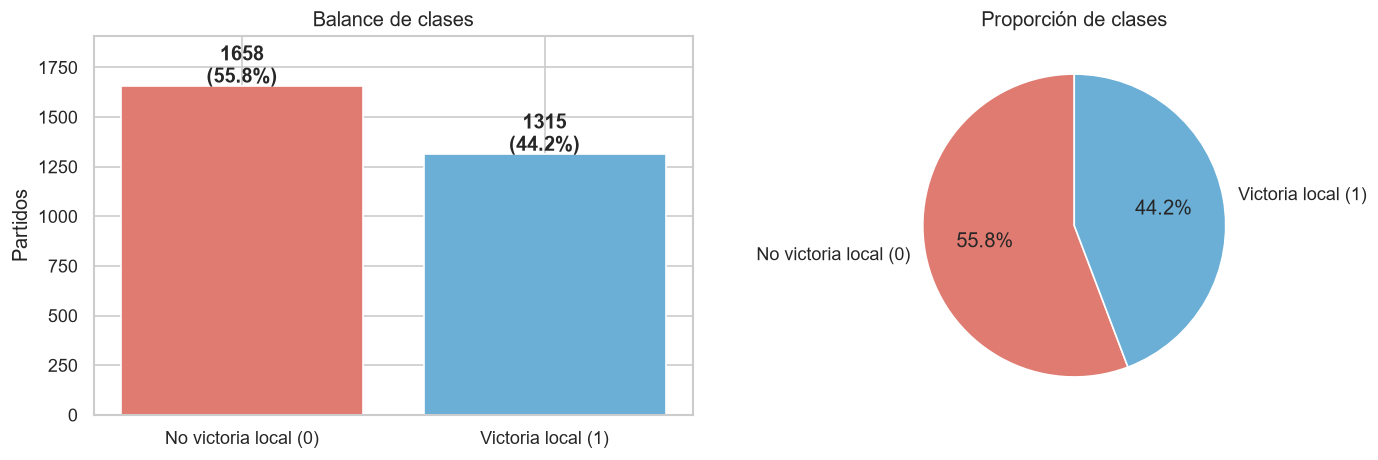
\includegraphics[width=0.7\textwidth]{figuras/eda/balance_clases.png}
\caption[Balance de clases de \texttt{target\_home\_win}]{Balance de clases de \texttt{target\_home\_win}. Fuente: elaboración propia con datos de FBref y football-data.co.uk.}
\label{fig:balance}
\end{figure}

\section{Feature engineering}
La construcción de variables fue iterativa, en tres versiones:
\begin{itemize}
\item \textbf{v1 (base):} forma \textit{rolling} (5 partidos), estadísticas de temporada y \textit{head-to-head}; replican y extienden las de Baboota y Kaur~\cite{baboota2019predictive}.
\item \textbf{v2 (reducción + interacción):} eliminación de variables redundantes por alta correlación ($r>0{,}85$) y creación de interacciones como \texttt{streak\_clash} (choque de rachas invictas) y \texttt{market\_form\_diff} (diferencia entre forma real e implícita del mercado).
\item \textbf{v3 (+jugadores):} calidad del plantel (\texttt{diff\_player\_quality}), edad media (\texttt{diff\_squad\_age}), porteros (\texttt{diff\_gk\_save\_pct}, \texttt{diff\_gk\_cs\_pct}), entradas ganadas (\texttt{diff\_team\_tkl\_per90}) e intercepciones (\texttt{diff\_team\_int\_per90}) por 90 minutos.
\end{itemize}
La Figura~\ref{fig:top_features} muestra el top-20 de variables por correlación de Pearson con el objetivo.

\begin{figure}[!htbp]
\centering
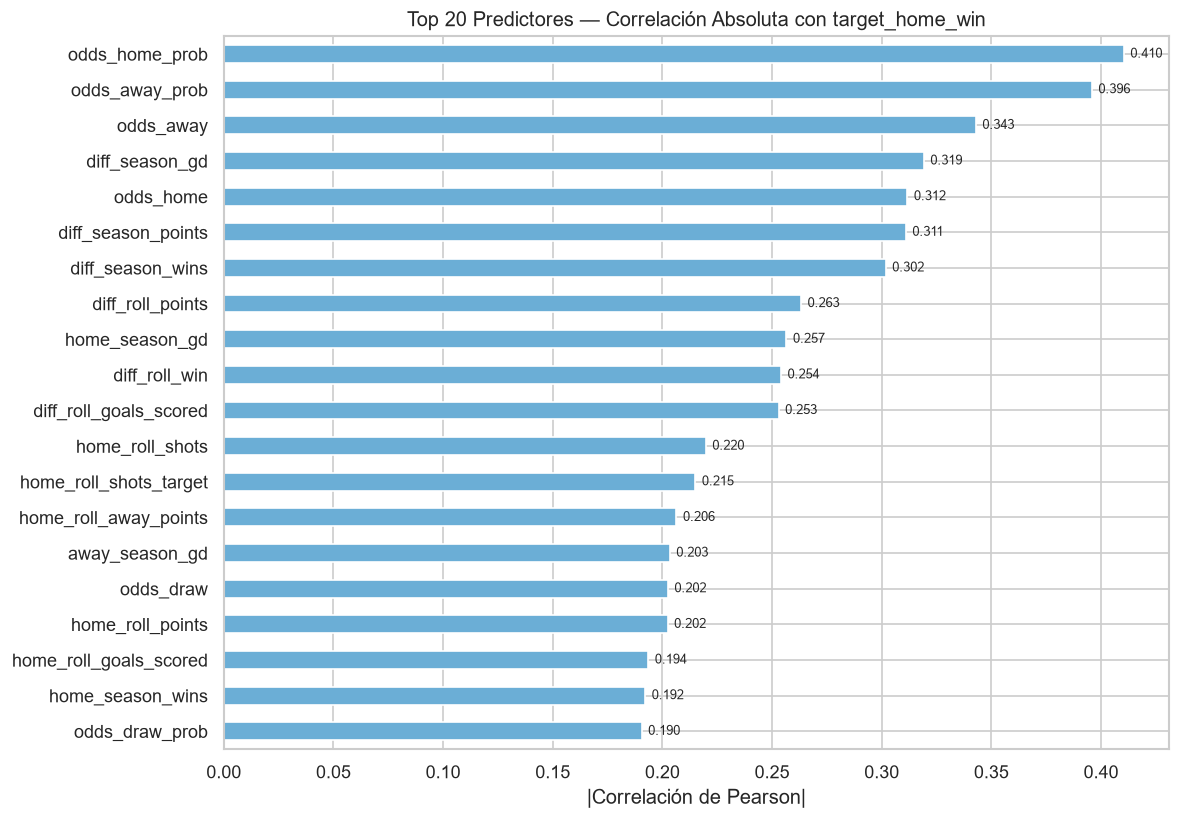
\includegraphics[width=0.7\textwidth]{figuras/eda/top_predictores.png}
\caption[Top-20 variables por correlación absoluta de Pearson con \texttt{target\_home\_win}]{Top-20 variables por correlación absoluta de Pearson con \texttt{target\_home\_win}. Fuente: elaboración propia con datos de FBref y football-data.co.uk.}
\label{fig:top_features}
\end{figure}

\section{Selección de variables}
Tras eliminar fuga de información (resultado, goles, identificadores) y redundancia (variables altamente correlacionadas, cuotas crudas, variables individuales de jugadores sustituidas por sus diferencias), quedaron 58 variables candidatas. Se aplicó \textit{Recursive Feature Elimination with Cross-Validation} (RFECV) con \texttt{TimeSeriesSplit} de 3 folds y Gradient Boosting como estimador base; el óptimo fue de \textbf{32 variables} (Figura~\ref{fig:rfecv}; F1 de validación cruzada 0,591). De ellas se descartaron 4 por colinealidad ($|r|>0{,}80$ con otra variable seleccionada: \texttt{odds\_away\_prob}, \texttt{home\_roll\_shots\_target}, \texttt{diff\_gk\_ga90} y \texttt{diff\_season\_gd}), quedando \textbf{28 variables}: 3 de mercado (\texttt{odds\_home\_prob}, \texttt{market\_form\_diff}, \texttt{market\_uncertainty}), 10 de forma y rachas, 3 de temporada, 2 de enfrentamientos directos y 10 de plantel y porteros. Con ellas el F1 de validación fue de 0,588 $\pm$ 0,041 y el ROC-AUC de 0,683 $\pm$ 0,030. La curva de RFECV es prácticamente plana (F1 entre 0,57 y 0,59 desde unas 10 variables hasta las 54), por lo que el número óptimo no está bien determinado: con muchas menos variables se obtiene casi el mismo desempeño, un primer indicio de que las variables adicionales aportan poco.

\begin{figure}[!htbp]
\centering
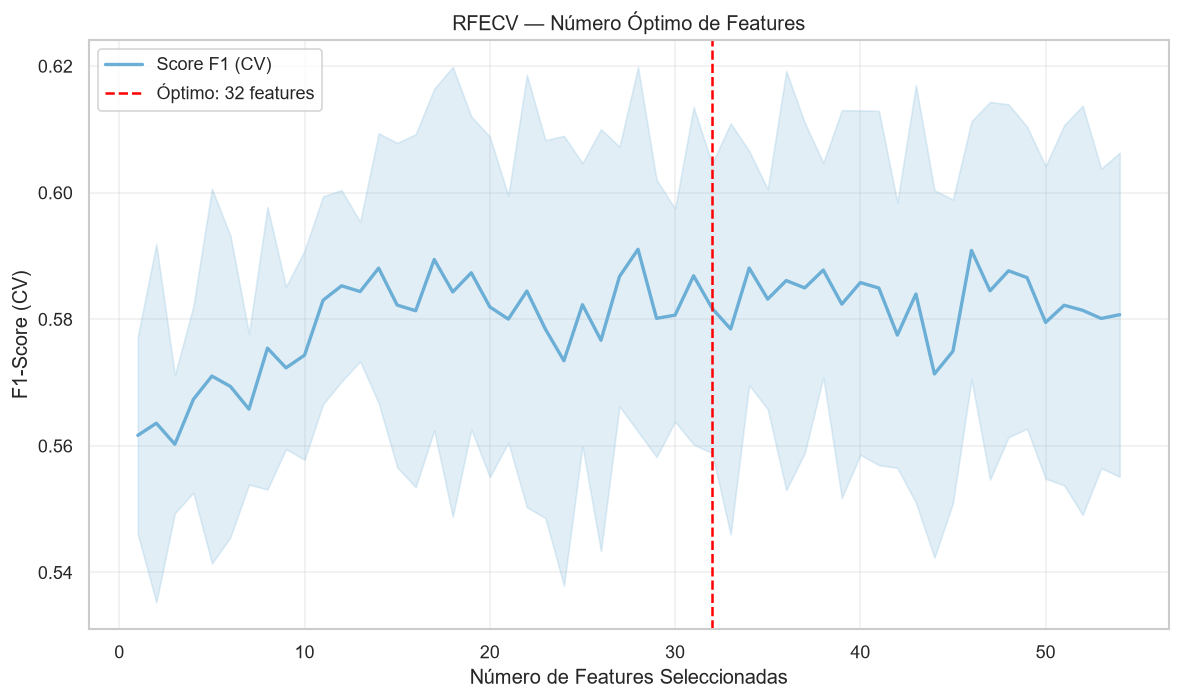
\includegraphics[width=0.7\textwidth]{figuras/feature_selection/rfecv_curve.png}
\caption[Curva de RFECV: número óptimo de variables seleccionadas (32, reducidas a 28 por colinealidad)]{Curva de RFECV: número óptimo de variables seleccionadas (32, reducidas a 28 por colinealidad). Fuente: elaboración propia con datos de FBref y football-data.co.uk.}
\label{fig:rfecv}
\end{figure}

\section{Modelos evaluados}
Se evaluaron siete algoritmos~\cite{geron2022hands}: \textbf{Gradient Boosting} (boosting secuencial de árboles débiles), \textbf{Random Forest} (\textit{bagging} de árboles con submuestreo de variables), \textbf{Regresión Logística}, \textbf{SVM con kernel RBF}, \textbf{MLP} de scikit-learn, una \textbf{red neuronal en PyTorch} (arquitectura $n\!\rightarrow\!256\!\rightarrow\!128\!\rightarrow\!64\!\rightarrow\!32\!\rightarrow\!1$ con BatchNorm, Dropout y \textit{early stopping}) y una \textbf{red neuronal en Keras optimizada con Keras Tuner}. Esta última explora 1 a 3 capas ocultas de 16 a 128 neuronas, tres funciones de activación, \textit{dropout}, regularización L2, tres optimizadores, tasa de aprendizaje y tamaño de lote, mediante optimización bayesiana con 20 configuraciones por fold. Para cada fold la búsqueda usa como validación el último 20\% cronológico del entrenamiento, de modo que el conjunto de test nunca interviene en la decisión; la red final se entrena sobre todo el entrenamiento y se promedian 10 redes con semillas distintas. Como referencia se incluye una regresión logística entrenada solo con las tres probabilidades implícitas de las cuotas (\textbf{solo cuotas}).

\section{Validación temporal y optimización}
Se usó validación de ventana expansiva (\textit{expanding window}) con 7 folds: el fold $k$ entrena con las primeras $k$ temporadas y evalúa en la siguiente (Fold 1: entrenamiento 2017--18, test 2018--19; \dots; Fold 7: entrenamiento 2017--24, test 2024--25). Los hiperparámetros se optimizaron con \texttt{GridSearchCV} y \texttt{TimeSeriesSplit} interno de 3 folds, con F1 como métrica; la red PyTorch se ajustó manualmente sobre tres configuraciones. En la etapa final de calibración y mezcla de modelos los hiperparámetros se eligieron por log-loss, sin pesos de clase y calibrando el Random Forest con el método sigmoide. Los modelos sensibles a la escala usan \texttt{StandardScaler} ajustado solo con el entrenamiento de cada fold.

\section{Métricas de evaluación}
Se usaron accuracy, F1-Score (útil ante el leve desbalance), ROC-AUC (capacidad discriminativa), Brier Score y log-loss (calidad de las probabilidades; menor es mejor). Con cerca de 370 partidos por temporada de test, el error estándar del accuracy en una temporada es de unos 2,4 puntos porcentuales, por lo que las diferencias menores a 1 punto no son concluyentes.

\section{Distribución del trabajo}
La Tabla~\ref{tab:tareas} resume las tareas realizadas por integrante hasta el primer informe.

\begin{table}[!htbp]
\caption[Tareas completadas por integrante (primer informe)]{Tareas completadas por integrante (primer informe).}
\label{tab:tareas}
\centering
\footnotesize
\setlength{\tabcolsep}{3pt}
\begin{tabular}{@{}p{1.9cm}p{1.7cm}p{4.2cm}@{}}
\toprule
\textbf{Responsable} & \textbf{Área} & \textbf{Tarea} \\
\midrule
Anakin Benavides & Datos & Recolección, limpieza y consolidación del dataset \\
Anakin Benavides & Feature Eng. & Forma \textit{rolling}, rachas, features de jugadores y porteros \\
Anakin Benavides & EDA & Distribuciones, correlaciones y top features \\
Anakin Benavides & Modelado & Pipeline de validación temporal \\
Sebastián Valdovinos & Modelado & Entrenamiento de los 6 modelos; iteración de versiones v1--v3 \\
Sebastián Valdovinos & Evaluación & Métricas, importancia Gini y baseline del mercado \\
\bottomrule
\end{tabular}
\par\smallskip{\footnotesize Fuente: elaboración propia.}
\end{table}

\chapter{RESULTADOS}
\label{sec:resultados}

\section{Resultados sin optimización de hiperparámetros}
La Tabla~\ref{tab:baseline} presenta las métricas iniciales de los seis modelos sin optimización, con partición cronológica 80/20 (595 partidos de test).

\begin{table}[!htbp]
\caption[Métricas en el conjunto de test sin optimización (partición 80/20)]{Métricas en el conjunto de test sin optimización (partición 80/20).}
\label{tab:baseline}
\centering
\footnotesize
\begin{tabular}{@{}lcccc@{}}
\toprule
\textbf{Modelo} & \textbf{Acc.} & \textbf{F1} & \textbf{AUC} & \textbf{Brier} \\
\midrule
Red neuronal PyTorch & 65,71\% & 0,6344 & 0,7454 & 0,2040 \\
Reg. Logística & 66,55\% & 0,6575 & 0,7415 & 0,2116 \\
Random Forest & 67,23\% & 0,6328 & 0,7322 & 0,2095 \\
MLP (sklearn) & 67,39\% & 0,6196 & 0,7321 & 0,2108 \\
SVM (RBF) & 66,39\% & 0,6441 & 0,7208 & 0,2123 \\
Gradient Boosting & 65,55\% & 0,5908 & 0,7060 & 0,2206 \\
\midrule
\textbf{Regla simple del mercado} & \textbf{64,26\%} & --- & --- & --- \\
\bottomrule
\end{tabular}
\par\smallskip{\footnotesize Fuente: elaboración propia con datos de FBref y football-data.co.uk.}
\end{table}

Todos los modelos superan a la regla simple del mercado, pero por márgenes pequeños (entre 1,3 y 3,1 puntos porcentuales). La Figura~\ref{fig:roc} muestra las curvas ROC.

\begin{figure}[!htbp]
\centering
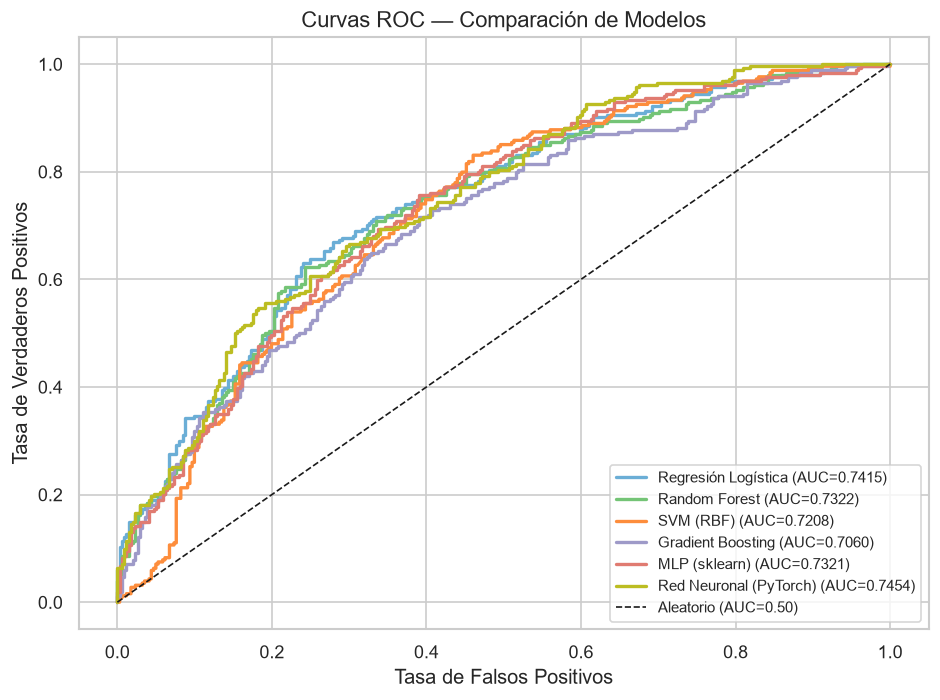
\includegraphics[width=0.7\textwidth]{figuras/modelos/curvas_roc.png}
\caption[Curvas ROC comparativas de los modelos sin optimización]{Curvas ROC comparativas de los modelos sin optimización. Fuente: elaboración propia con datos de FBref y football-data.co.uk.}
\label{fig:roc}
\end{figure}

\section{Resultados con optimización de hiperparámetros}
La Tabla~\ref{tab:tuning} presenta los resultados promediados sobre los 7 folds (media $\pm$ desviación estándar), ordenados por ROC-AUC. La regla simple del mercado alcanza 64,4\% en las mismas temporadas.

\begin{table}[!htbp]
\caption[Resultados con optimización de hiperparámetros (7 folds)]{Resultados con optimización de hiperparámetros (7 folds).}
\label{tab:tuning}
\centering
\footnotesize
\setlength{\tabcolsep}{2pt}
\begin{tabular}{@{}lcccc@{}}
\toprule
\textbf{Modelo} & \textbf{Acc.} & \textbf{F1} & \textbf{AUC} & \textbf{Brier} \\
\midrule
Solo cuotas (Reg. Log.) & 67,67 $\pm$ 1,0\% & 0,636 & 0,736 $\pm$ 0,019 & 0,208 \\
Reg. Logística & 67,44 $\pm$ 1,2\% & 0,641 & 0,731 $\pm$ 0,023 & 0,212 \\
Random Forest & 68,24 $\pm$ 1,2\% & 0,628 & 0,727 $\pm$ 0,021 & 0,211 \\
Red neuronal PyTorch & 68,01 $\pm$ 0,9\% & 0,627 & 0,725 $\pm$ 0,014 & 0,211 \\
Red Keras Tuner & 66,82 $\pm$ 2,1\% & 0,601 & 0,716 $\pm$ 0,025 & 0,217 \\
Gradient Boosting & 65,80 $\pm$ 3,0\% & 0,590 & 0,704 $\pm$ 0,039 & 0,224 \\
MLP (sklearn) & 65,76 $\pm$ 2,7\% & 0,581 & 0,703 $\pm$ 0,040 & 0,227 \\
SVM (RBF) & 61,07 $\pm$ 8,4\% & 0,618 & 0,690 $\pm$ 0,039 & 0,225 \\
\bottomrule
\end{tabular}
\par\smallskip{\footnotesize Fuente: elaboración propia con datos de FBref y football-data.co.uk.}
\end{table}

Random Forest obtiene el mayor accuracy (68,24\%, +3,9 puntos sobre la regla simple, y la supera en los 7 folds), seguido de la red PyTorch y de la regresión logística (+3,1 puntos, también en los 7 folds); Gradient Boosting solo la supera por 1,4 puntos y en 6 de 7 folds. Sin embargo, el mejor ROC-AUC lo obtiene la regresión logística que usa únicamente las tres probabilidades de las cuotas (0,736), por encima de todos los modelos con 28 variables. Las diferencias entre Random Forest, la red PyTorch y la regresión logística son menores que la desviación entre folds. La Figura~\ref{fig:comparacion_final} compara las métricas y la Figura~\ref{fig:folds} su evolución por fold.

\begin{figure}[!htbp]
\centering
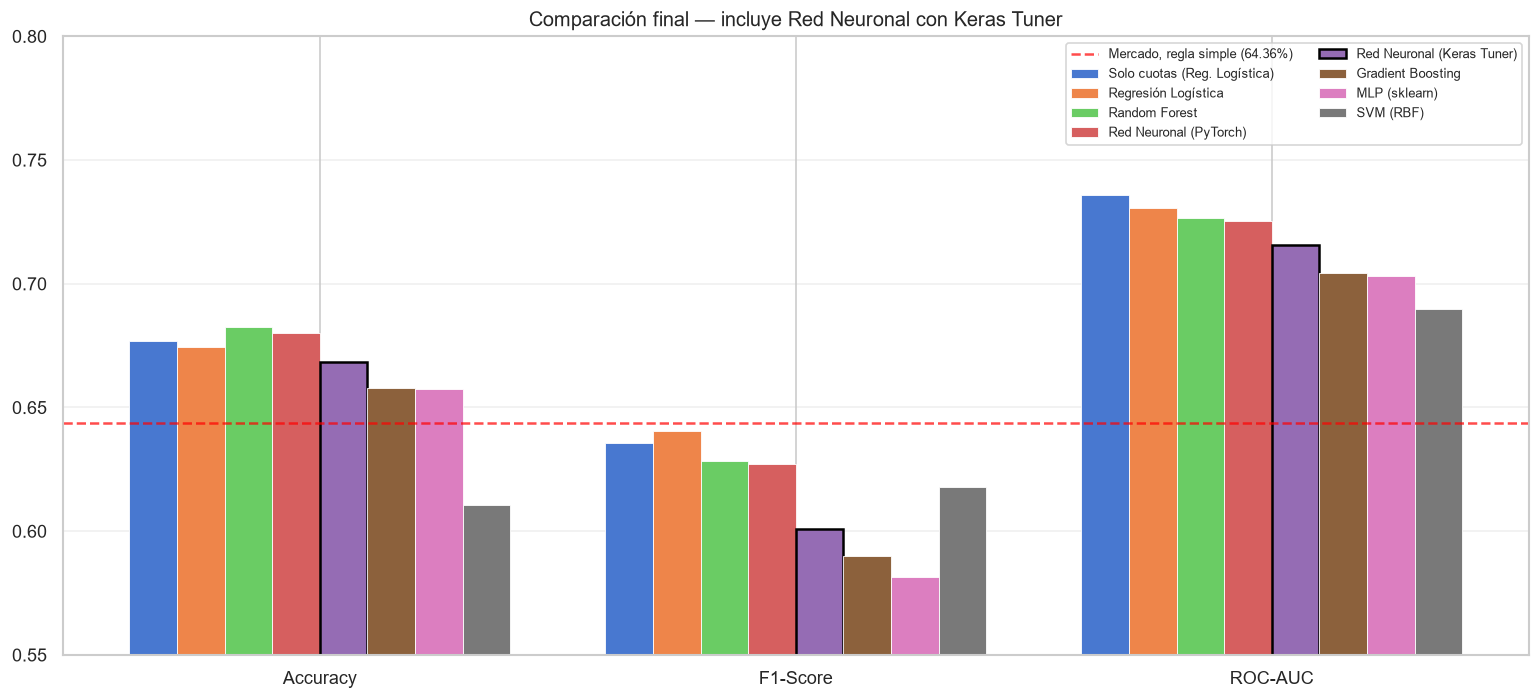
\includegraphics[width=0.8\textwidth]{figuras/keras_tuner/comparacion_final.png}
\caption[Comparación final de modelos (promedio de 7 folds) frente a la regla simple del mercado]{Comparación final de modelos (promedio de 7 folds) frente a la regla simple del mercado. Fuente: elaboración propia con datos de FBref y football-data.co.uk.}
\label{fig:comparacion_final}
\end{figure}

\begin{figure}[!htbp]
\centering
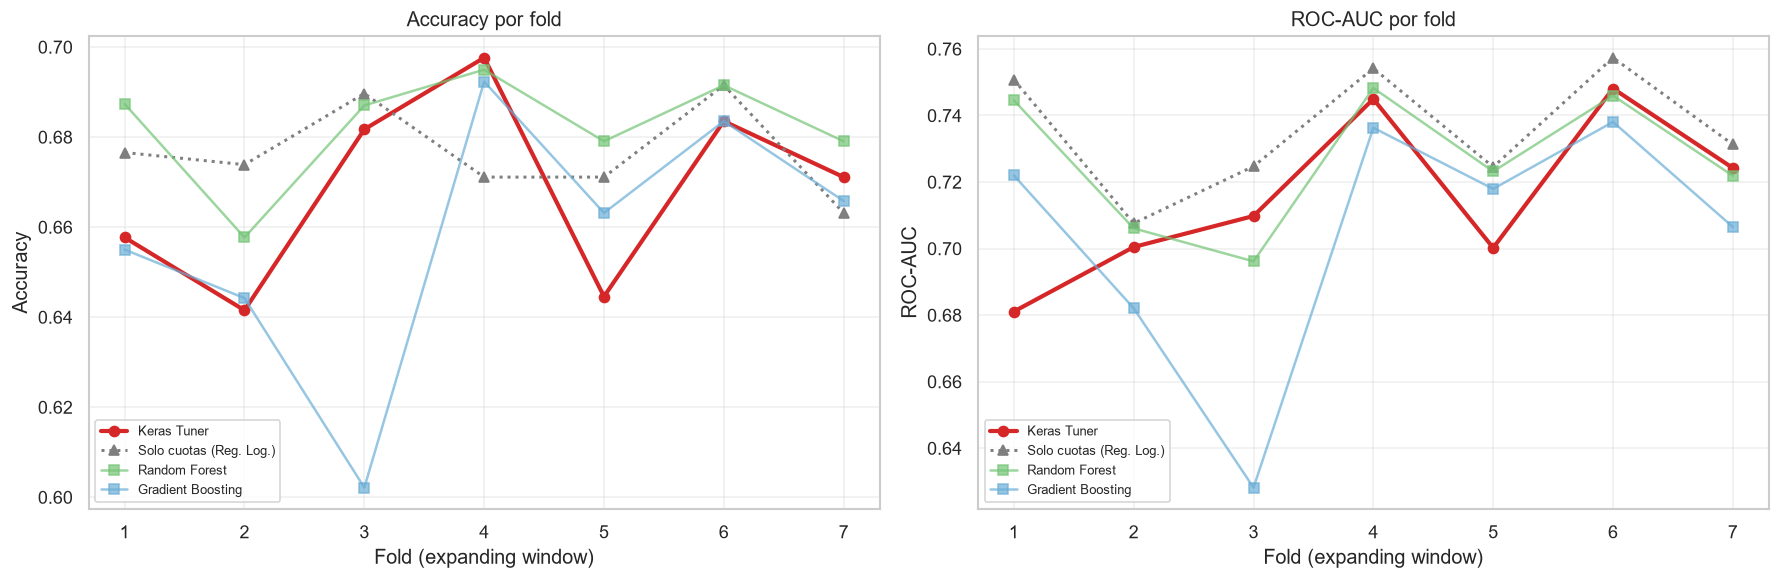
\includegraphics[width=0.8\textwidth]{figuras/keras_tuner/evolucion_folds.png}
\caption[Evolución de accuracy y ROC-AUC por fold de validación]{Evolución de accuracy y ROC-AUC por fold de validación. Fuente: elaboración propia con datos de FBref y football-data.co.uk.}
\label{fig:folds}
\end{figure}

\section{Red neuronal con Keras Tuner}
La búsqueda bayesiana no converge a una arquitectura estable: las mejores configuraciones por fold van desde 1 hasta 3 capas, con 16 a 112 neuronas en la primera y distintas activaciones y optimizadores, y las épocas óptimas varían entre 4 y 40. Es el comportamiento esperable con cerca de 2.900 filas, donde el espacio de búsqueda es prácticamente plano. Una primera ejecución, con una sola red por fold, resultó muy inestable (63,3\% $\pm$ 10,0 de accuracy): en el fold 1, con solo 347 partidos de entrenamiento, el accuracy fue de 41,2\% y el AUC de 0,44. El diagnóstico mostró que no era un error de datos sino varianza de inicialización: la misma configuración entrenada con 10 semillas dio AUC entre 0,44 y 0,72 en ese fold. Se adoptó entonces promediar 10 redes por fold, medida aplicada por igual a los 7 folds y no basada en elegir la mejor semilla. Con ello la red alcanza 66,8\% $\pm$ 2,1 de accuracy y 0,716 de AUC. Debe señalarse que esta decisión se tomó \textit{después} de observar el fold 1; la primera ejecución se conserva en el repositorio.

\section{Importancia de variables}
La importancia por permutación de Gradient Boosting (último fold) muestra que \texttt{odds\_home\_prob} domina por amplio margen (0,133 de reducción de F1 al permutarla), mientras que 24 de las 28 variables tienen una importancia menor o igual a 0,005, y varias negativa. La importancia Gini de los modelos de árboles lleva a la misma conclusión (Figura~\ref{fig:feature_importance}). Un análisis combinado de tres criterios (Gini, permutación y coeficientes de la regresión logística) dejó 12 variables candidatas a eliminar; al quitar cada una por separado el F1 mejora entre 0,006 y 0,016 en 10 de ellas (Figura~\ref{fig:elimination}), un orden de magnitud similar al ruido entre folds. El conjunto reducido de 18 variables resultante no se usó en los modelos finales, que conservan las 28.

\begin{figure}[!htbp]
\centering
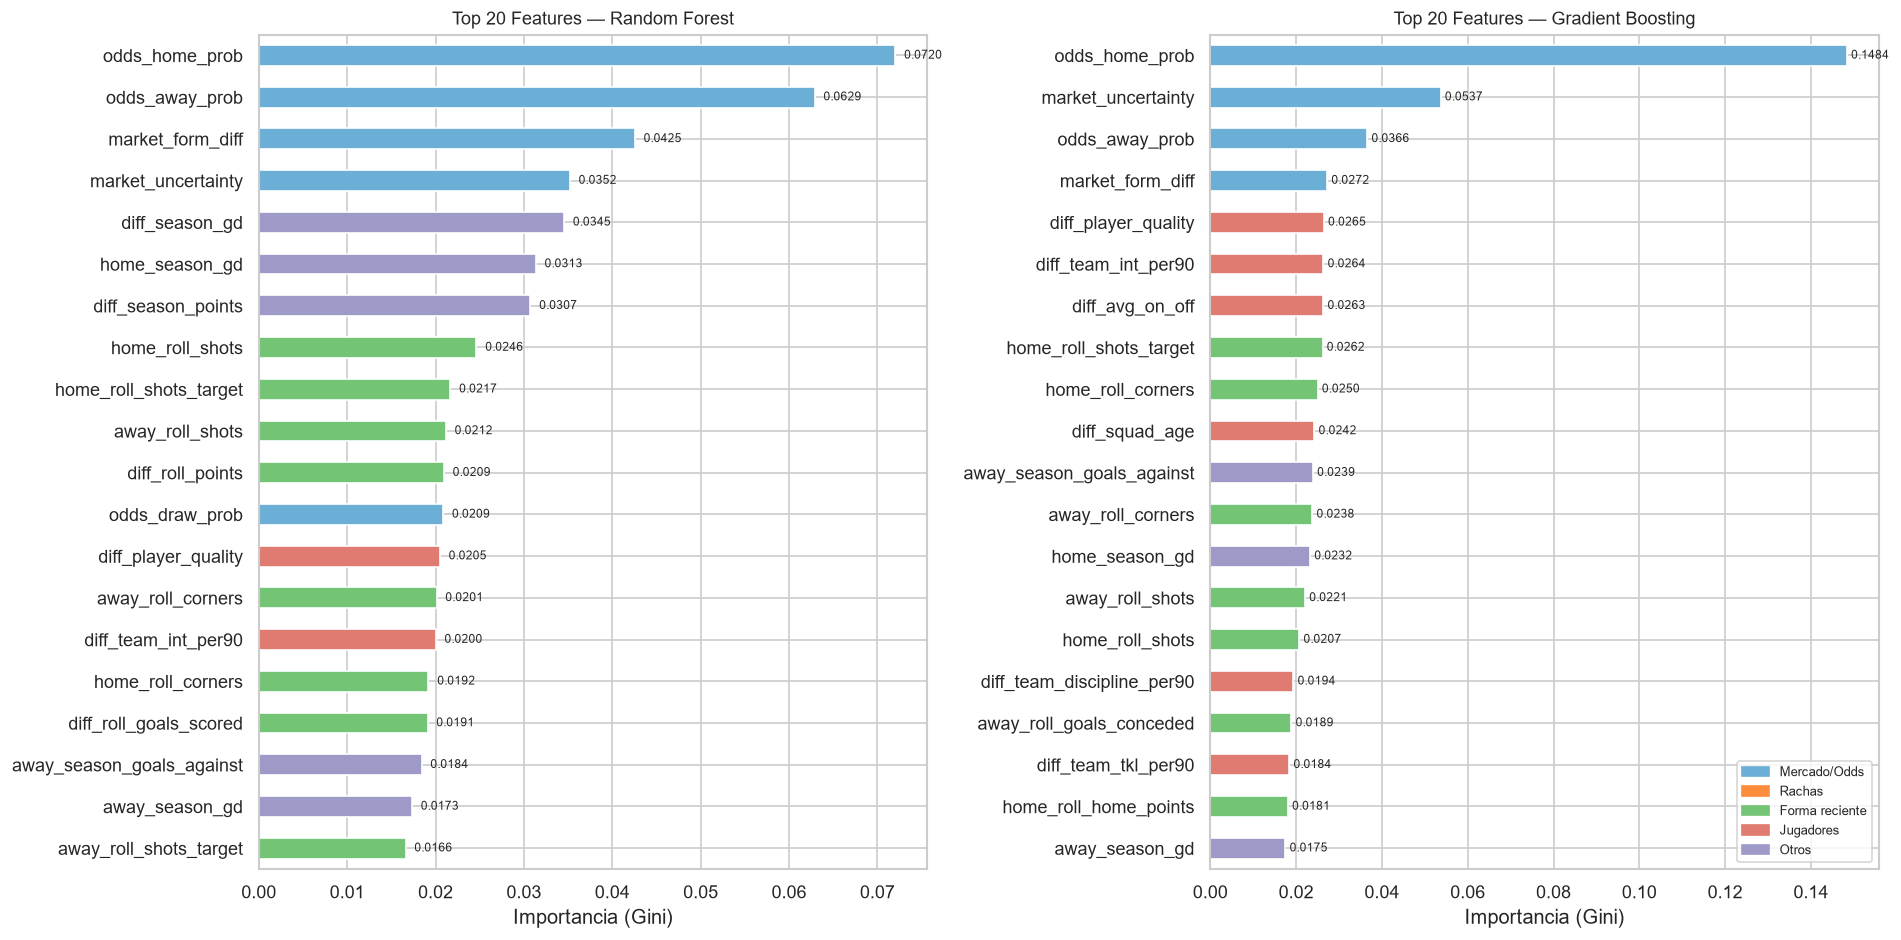
\includegraphics[width=0.8\textwidth]{figuras/tuning/feature_importance.png}
\caption[Importancia de variables (Gini) para Random Forest y Gradient Boosting]{Importancia de variables (Gini) para Random Forest y Gradient Boosting. Fuente: elaboración propia con datos de FBref y football-data.co.uk.}
\label{fig:feature_importance}
\end{figure}

\begin{figure}[!htbp]
\centering
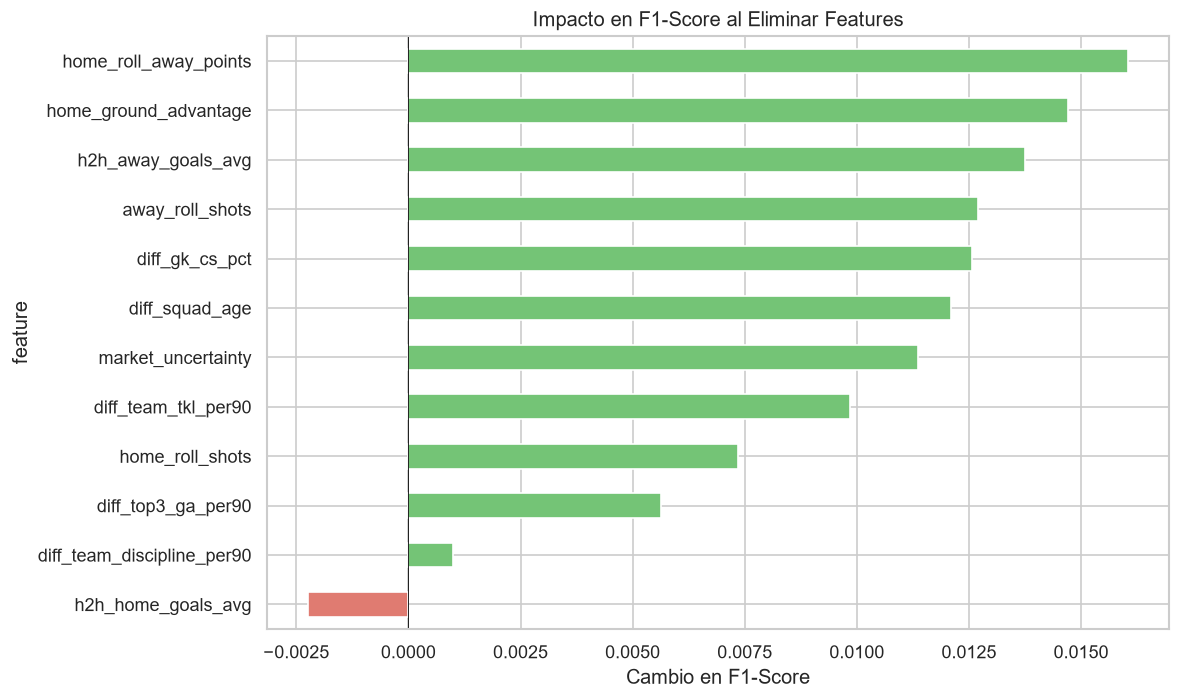
\includegraphics[width=0.7\textwidth]{figuras/features_negativos/elimination_impact.png}
\caption[Impacto sobre el F1-Score de eliminar cada variable candidata (3 primeros folds)]{Impacto sobre el F1-Score de eliminar cada variable candidata (3 primeros folds). Fuente: elaboración propia con datos de FBref y football-data.co.uk.}
\label{fig:elimination}
\end{figure}

\section{Análisis sin variables de mercado}
Se eliminaron tres variables de mercado (\texttt{odds\_home\_prob}, \texttt{market\_form\_diff}, \texttt{market\_uncertainty}) para evaluar si los modelos dependen de las cuotas (Tabla~\ref{tab:sin_odds}, Figura~\ref{fig:sin_odds}).

\begin{table}[!htbp]
\caption[Accuracy con y sin variables de mercado (promedio de 7 folds, hiperparámetros fijos)]{Accuracy con y sin variables de mercado (promedio de 7 folds, hiperparámetros fijos).}
\label{tab:sin_odds}
\centering
\footnotesize
\begin{tabular}{@{}lccc@{}}
\toprule
\textbf{Modelo} & \textbf{Con odds} & \textbf{Sin odds} & \textbf{Caída} \\
\midrule
Random Forest & 68,31\% & 64,93\% & $-$3,38 pp \\
Reg. Logística & 67,21\% & 64,80\% & $-$2,41 pp \\
MLP (sklearn) & 66,29\% & 64,18\% & $-$2,11 pp \\
Gradient Boosting & 64,42\% & 62,67\% & $-$1,75 pp \\
SVM (RBF) & 64,29\% & 62,84\% & $-$1,45 pp \\
\bottomrule
\end{tabular}
\par\smallskip{\footnotesize Fuente: elaboración propia con datos de FBref y football-data.co.uk.}
\end{table}

\begin{figure}[!htbp]
\centering
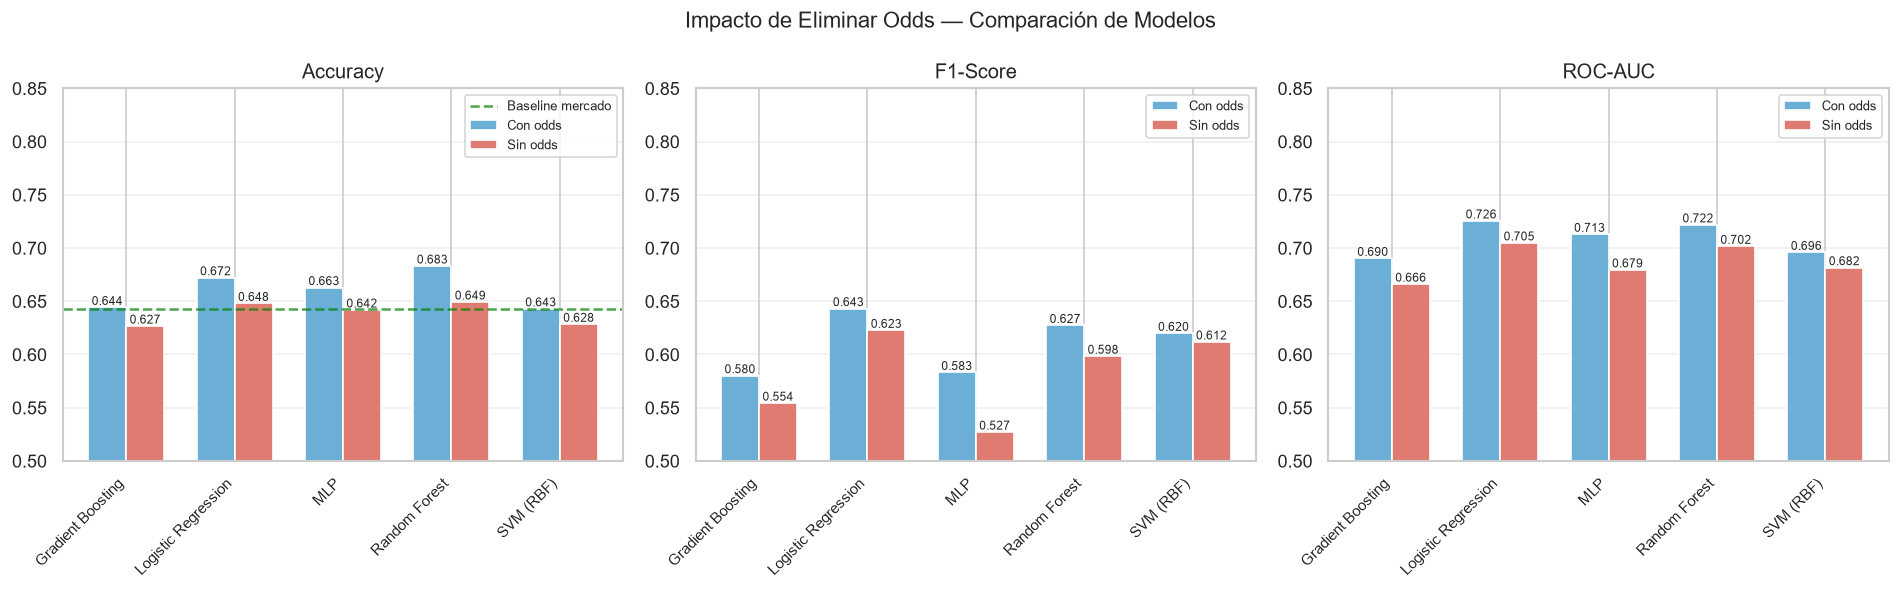
\includegraphics[width=0.8\textwidth]{figuras/sin_odds/comparacion_odds.png}
\caption[Impacto de eliminar las variables de mercado sobre accuracy, F1 y ROC-AUC]{Impacto de eliminar las variables de mercado sobre accuracy, F1 y ROC-AUC. Fuente: elaboración propia con datos de FBref y football-data.co.uk.}
\label{fig:sin_odds}
\end{figure}

La caída promedio de accuracy es de 2,22 puntos porcentuales. Sin cuotas, el mejor modelo (Random Forest, 64,93\%) solo iguala a la regla simple del mercado (64,4\%, +0,6 puntos) y queda unos 3,7 puntos por debajo de la regresión logística sobre las cuotas. Es decir, las variables de forma, plantel y enfrentamientos directos no logran reemplazar la información que incorporan las cuotas. Los valores con odds difieren de la Tabla~\ref{tab:tuning} porque aquí se usan hiperparámetros fijos, no optimizados por fold.

\section{Calibración y mezcla de modelos}
Hasta aquí los modelos usaban \texttt{class\_weight='balanced'} y se afinaban por F1, lo que distorsiona las probabilidades. Se repitió la evaluación optimizando por calidad de probabilidad: sin pesos de clase, hiperparámetros elegidos por log-loss con validación temporal interna y Random Forest calibrado. Además se evaluó una mezcla por promedio simple de tres modelos (solo cuotas, regresión logística y Random Forest). El criterio de éxito se fijó antes de ver los resultados: la mezcla debía mejorar el log-loss en las temporadas de desarrollo (folds 1 a 4) y confirmarlo en las tres últimas (folds 5 a 7). La Tabla~\ref{tab:mezcla} resume el resultado.

\begin{table}[!htbp]
\caption[Modelos calibrados y mezcla (promedio de 7 folds)]{Modelos calibrados y mezcla (promedio de 7 folds).}
\label{tab:mezcla}
\centering
\footnotesize
\setlength{\tabcolsep}{2pt}
\begin{tabular}{@{}lcccc@{}}
\toprule
\textbf{Modelo} & \textbf{Log-loss} & \textbf{AUC} & \textbf{Brier} & \textbf{Acc.} \\
\midrule
Solo cuotas & 0,598 & 0,736 & 0,206 & 68,58\% \\
Mezcla (promedio simple) & 0,602 & 0,735 & 0,207 & 68,47\% \\
Random Forest calibrado & 0,608 & 0,727 & 0,210 & 68,28\% \\
Reg. Logística (28 variables) & 0,610 & 0,730 & 0,211 & 68,55\% \\
\bottomrule
\end{tabular}
\par\smallskip{\footnotesize Fuente: elaboración propia con datos de FBref y football-data.co.uk.}
\end{table}

El criterio \textbf{no se cumplió}: la mezcla supera al Random Forest y a la regresión logística por separado (en 6 y 7 de los 7 folds en log-loss), pero no supera a la regresión sobre las cuotas, que mejora en 6 de 7 folds. Quitar los pesos de clase sí elevó el accuracy de la regresión sobre cuotas de 67,7\% a 68,6\% y el de la regresión logística de 67,4\% a 68,6\%, pero todos los modelos quedaron en el mismo rango (68,3 a 68,6\%), que es el techo que impone la información de las cuotas (Figura~\ref{fig:mezcla}).

\begin{figure}[!htbp]
\centering
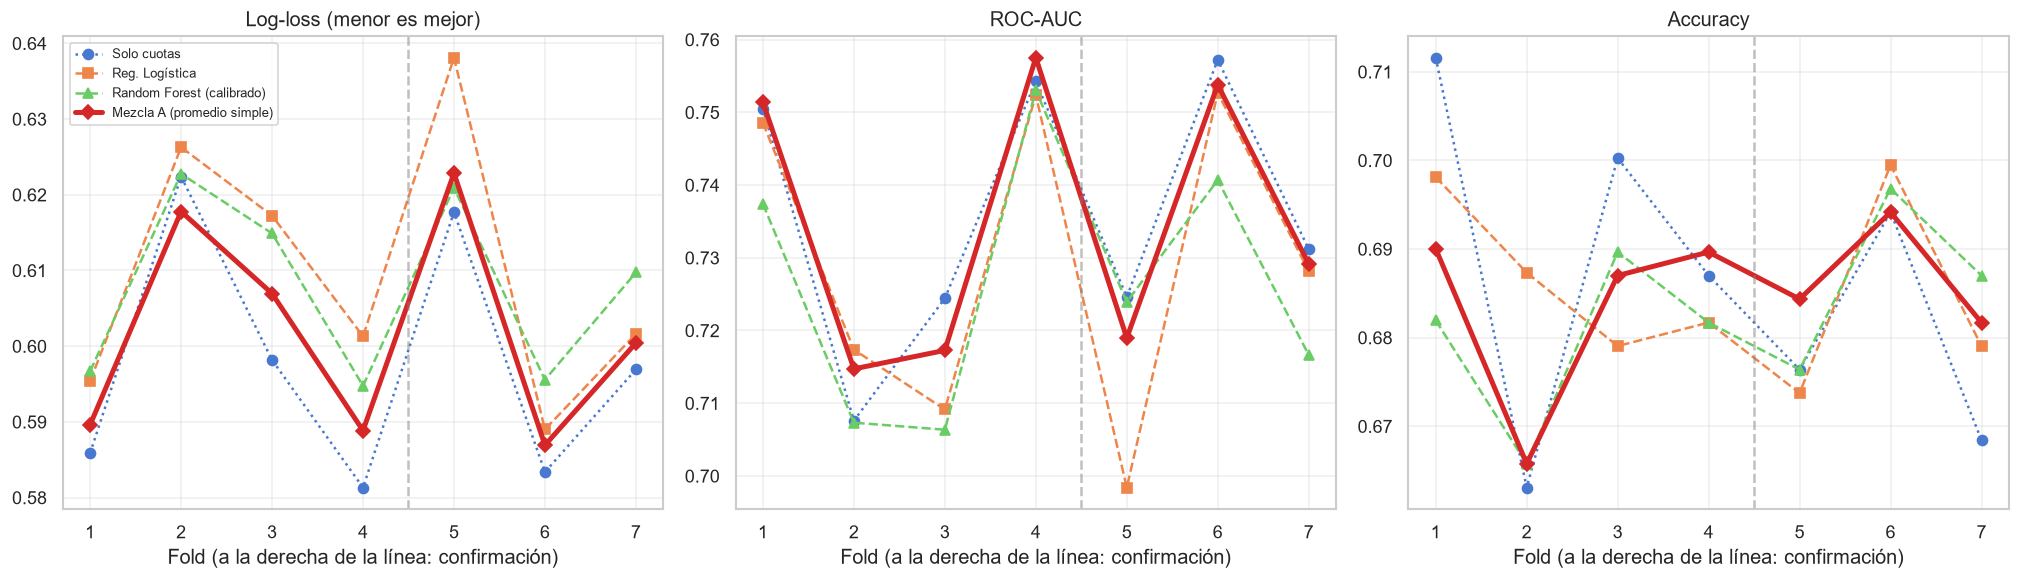
\includegraphics[width=0.8\textwidth]{figuras/mezcla_modelos/comparacion_folds.png}
\caption[Log-loss, ROC-AUC y accuracy por fold de los modelos calibrados y de la mezcla (a la derecha de la línea, temporadas de confirmación)]{Log-loss, ROC-AUC y accuracy por fold de los modelos calibrados y de la mezcla (a la derecha de la línea, temporadas de confirmación). Fuente: elaboración propia con datos de FBref y football-data.co.uk.}
\label{fig:mezcla}
\end{figure}

\section{Interpretabilidad con valores SHAP}
\label{sec:shap}
Los valores SHAP~\cite{lundberg2017unified} descomponen cada predicción en contribuciones aditivas de cada variable, $f(x)=\phi_0+\sum_{j}\phi_j$, donde $\phi_0$ es el valor base y $\phi_j$ el aporte de la variable $j$ en log-odds. Se aplicó \texttt{TreeExplainer} a Gradient Boosting: en cada fold el modelo se entrenó solo con el pasado y los valores se calcularon sobre la temporada de test, de modo que la explicación refleja el comportamiento fuera de muestra. La Tabla~\ref{tab:shap} y la Figura~\ref{fig:shap_global} muestran las diez variables de mayor importancia global.

\begin{table}[!htbp]
\caption[Importancia global SHAP, 10 principales variables (media de $|\phi|$, promedio $\pm$ desv. est. entre 7 folds)]{Importancia global SHAP, 10 principales variables (media de $|\phi|$, promedio $\pm$ desv. est. entre 7 folds).}
\label{tab:shap}
\centering
\footnotesize
\begin{tabular}{@{}lc@{}}
\toprule
\textbf{Variable} & \textbf{Media $|$SHAP$|$} \\
\midrule
\texttt{odds\_home\_prob} & 0,656 $\pm$ 0,144 \\
\texttt{away\_roll\_corners} & 0,207 $\pm$ 0,124 \\
\texttt{home\_roll\_shots} & 0,186 $\pm$ 0,136 \\
\texttt{home\_season\_gd} & 0,171 $\pm$ 0,061 \\
\texttt{away\_roll\_shots} & 0,168 $\pm$ 0,113 \\
\texttt{away\_season\_goals\_against} & 0,164 $\pm$ 0,112 \\
\texttt{home\_ground\_advantage} & 0,164 $\pm$ 0,103 \\
\texttt{market\_uncertainty} & 0,154 $\pm$ 0,066 \\
\texttt{home\_roll\_corners} & 0,139 $\pm$ 0,086 \\
\texttt{home\_roll\_home\_points} & 0,139 $\pm$ 0,073 \\
\bottomrule
\end{tabular}
\par\smallskip{\footnotesize Fuente: elaboración propia con datos de FBref y football-data.co.uk.}
\end{table}

\begin{figure}[!htbp]
\centering
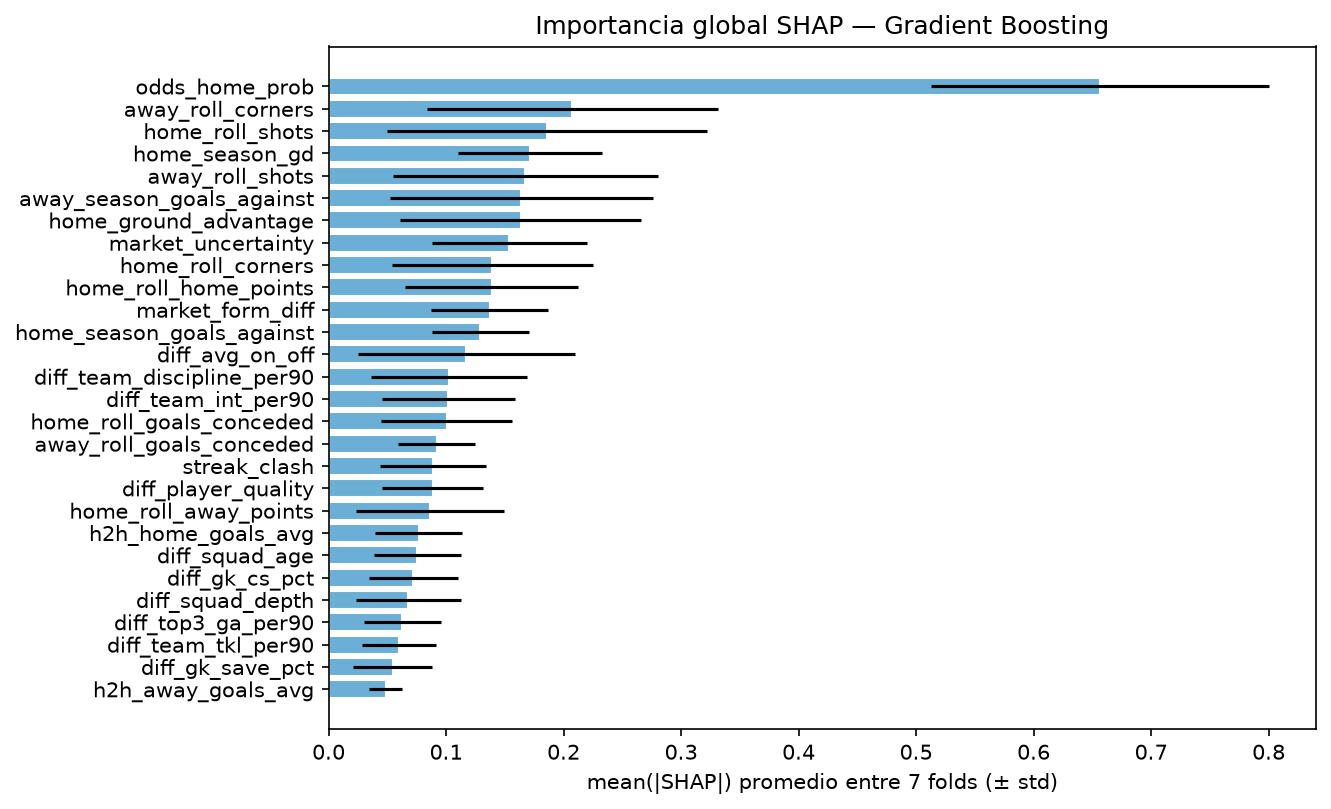
\includegraphics[width=0.7\textwidth]{figuras/shap/importancia_global.png}
\caption[Importancia global SHAP de Gradient Boosting (promedio de 7 folds)]{Importancia global SHAP de Gradient Boosting (promedio de 7 folds). Fuente: elaboración propia con datos de FBref y football-data.co.uk.}
\label{fig:shap_global}
\end{figure}

La probabilidad implícita del mercado domina: su aporte medio es más de tres veces el de la siguiente variable. El gráfico \textit{beeswarm} (Figura~\ref{fig:beeswarm}) muestra el sentido del efecto: valores altos de \texttt{odds\_home\_prob}, de los tiros recientes del local y de la diferencia de gol del local en la temporada aumentan la probabilidad de victoria local, mientras que más córners recientes del visitante la reducen. El resto de las variables aporta efectos pequeños y poco consistentes entre folds, lo que concuerda con el análisis de permutación y con la regresión sobre las cuotas.

\begin{figure}[!htbp]
\centering
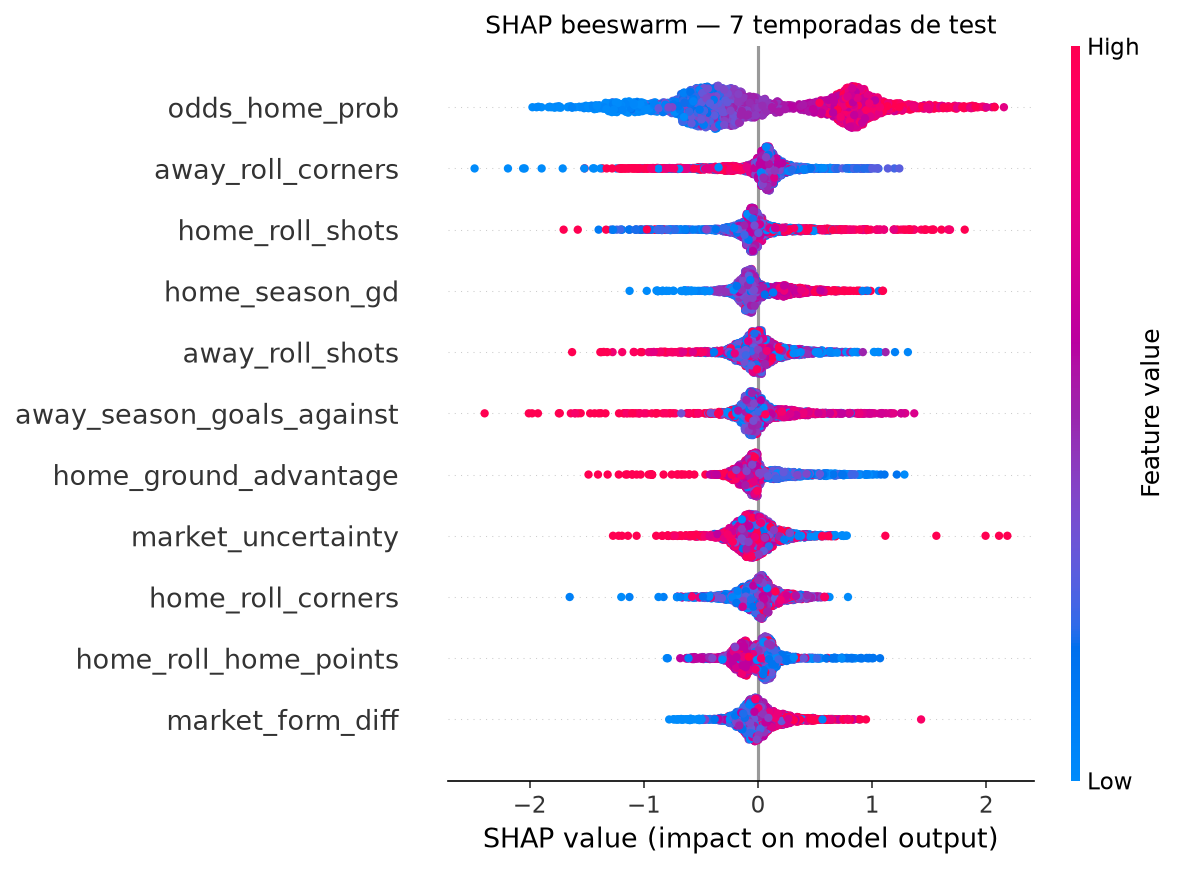
\includegraphics[width=0.8\textwidth]{figuras/shap/beeswarm.png}
\caption[SHAP \textit{beeswarm}: efecto de cada variable sobre la predicción en las 7 temporadas de test]{SHAP \textit{beeswarm}: efecto de cada variable sobre la predicción en las 7 temporadas de test. Fuente: elaboración propia con datos de FBref y football-data.co.uk.}
\label{fig:beeswarm}
\end{figure}

A nivel de partido, la Figura~\ref{fig:waterfall_err} muestra un error de alta confianza de la temporada 2024--25: Liverpool contra Crystal Palace (25 de mayo de 2025). El modelo asignó 0,94 de probabilidad de victoria local, impulsado principalmente por la cuota (\texttt{odds\_home\_prob} = 0,714, aporte de +0,95), la diferencia entre forma y mercado (+0,51) y los goles recibidos por el visitante en la temporada (+0,50); el partido terminó 1--1. El caso ilustra que el modelo no incorpora información contextual no estructurada, como lesiones, rotaciones o motivación al final de la temporada.

\begin{figure}[!htbp]
\centering
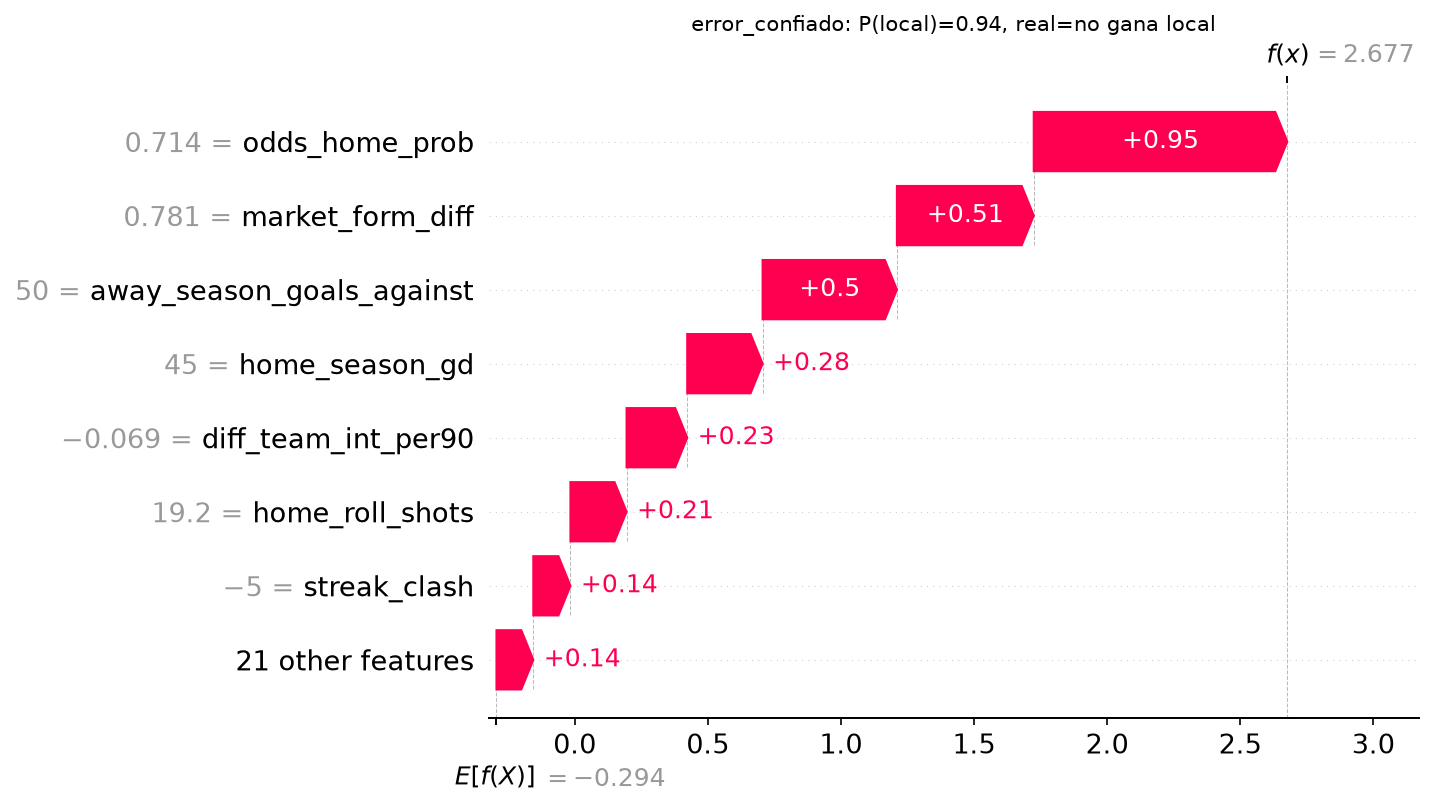
\includegraphics[width=0.8\textwidth]{figuras/shap/waterfall_error_confiado.png}
\caption[Explicación SHAP de un error de alta confianza (Liverpool--Crystal Palace, 2024--25)]{Explicación SHAP de un error de alta confianza (Liverpool--Crystal Palace, 2024--25). Fuente: elaboración propia con datos de FBref y football-data.co.uk.}
\label{fig:waterfall_err}
\end{figure}

\section{Prueba con datos reales: temporada 2025--26}
\label{sec:real}
Para verificar la generalización más allá del esquema de validación, se evaluaron los modelos sobre la temporada 2025--26, que no se usó en ninguna decisión del proyecto (selección de variables, hiperparámetros ni mezcla de modelos). Los resultados, estadísticas y cuotas se descargaron de football-data.co.uk y se procesaron con el mismo código del proyecto; un control confirmó que los partidos de 2017--2025 no cambian al agregar la temporada nueva, que la forma reciente coincide con un recálculo independiente que solo usa partidos anteriores, y que las medianas de imputación se calculan sin los partidos de prueba. Se excluyeron tres partidos del Sunderland, equipo recién ascendido sin historial en la liga, quedando 377 partidos. Random Forest (hiperparámetros elegidos por \textit{GridSearchCV} con ventana temporal) y la regresión logística sobre las tres cuotas se entrenaron una sola vez con las 2.973 observaciones de 2017--2025. La Tabla~\ref{tab:real} resume los resultados.

\begin{table}[!htbp]
\caption[Prueba con la temporada 2025--26 (377 partidos). Entre paréntesis, intervalo de confianza de Wilson del 95\% para el accuracy]{Prueba con la temporada 2025--26 (377 partidos). Entre paréntesis, intervalo de confianza de Wilson del 95\% para el accuracy.}
\label{tab:real}
\centering
\footnotesize
\begin{tabular}{@{}lccc@{}}
\toprule
\textbf{Modelo} & \textbf{Accuracy} & \textbf{ROC-AUC} & \textbf{Log-loss} \\
\midrule
Random Forest & 61,3\% (56,3--66,1) & 0,672 & 0,636 \\
Solo cuotas (reg. logística) & 62,9\% (57,9--67,6) & 0,697 & 0,619 \\
Regla simple del mercado & 60,5\% (55,5--65,3) & --- & --- \\
\bottomrule
\end{tabular}
\par\smallskip{\footnotesize Fuente: elaboración propia con datos de FBref y football-data.co.uk.}
\end{table}

\begin{figure}[!htbp]
\centering
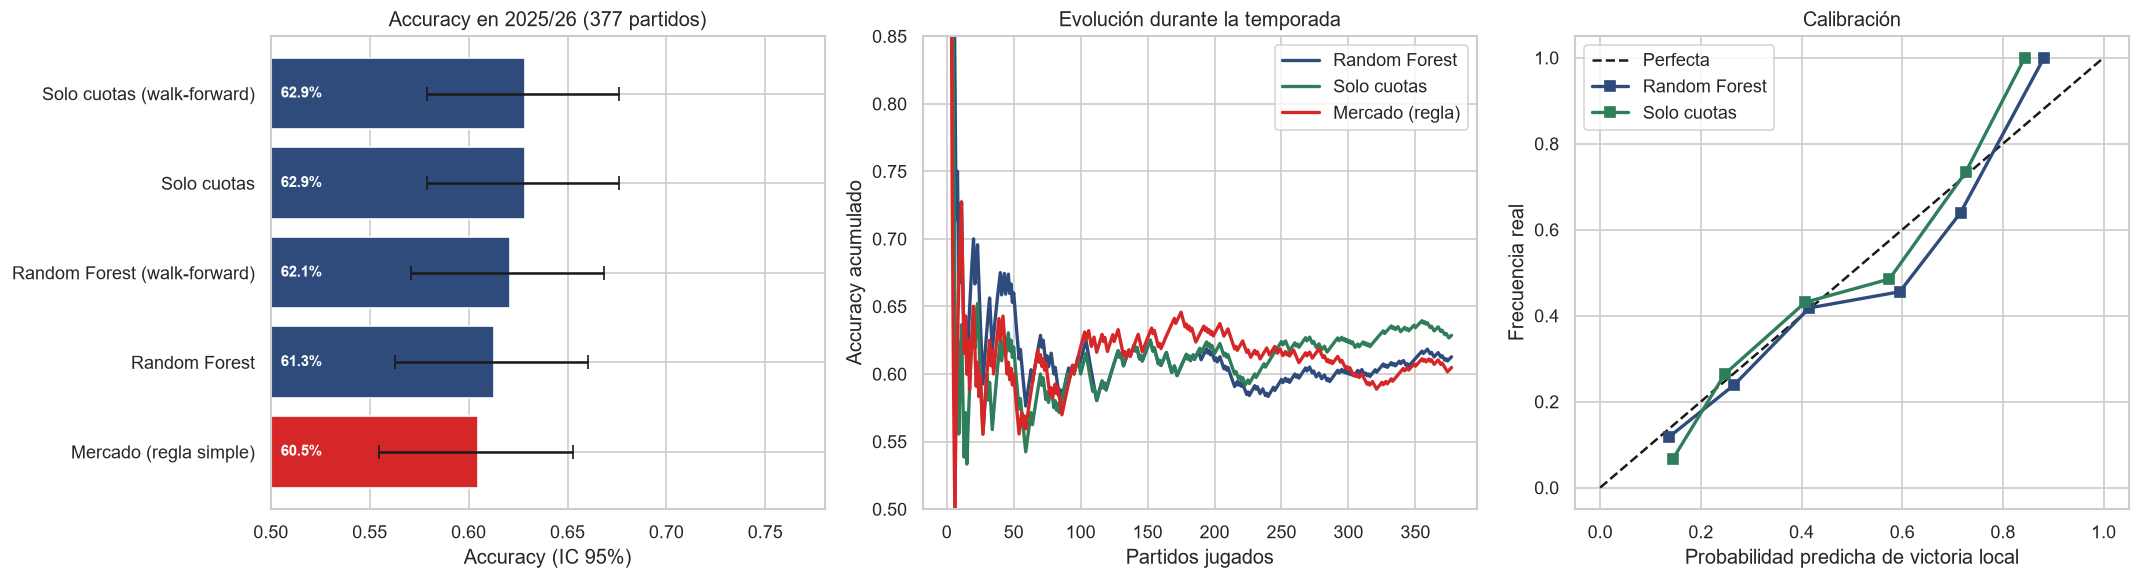
\includegraphics[width=0.8\textwidth]{figuras/prueba_real/resumen_2025_26.png}
\caption[Resultados de la prueba con la temporada 2025--26]{Resultados de la prueba con la temporada 2025--26. Fuente: elaboración propia con datos de FBref y football-data.co.uk.}
\label{fig:real}
\end{figure}

El rendimiento es menor que el promedio de los 7 folds (68,2\% y 67,7\%), pero los intervalos de confianza son de unos $\pm$5 puntos y ninguna diferencia es estadísticamente significativa según la prueba exacta de McNemar: Random Forest frente al mercado, $+0{,}8$ puntos ($p=0{,}83$); solo cuotas frente al mercado, $+2{,}4$ puntos ($p=0{,}41$); Random Forest frente a solo cuotas, $-1{,}6$ puntos ($p=0{,}34$). Reentrenar el Random Forest por bloques de partidos (\textit{walk-forward}) tampoco cambió el resultado (62,1\%). Por lo tanto, la prueba confirma la conclusión central: los modelos no superan de forma demostrable al mercado fuera de muestra. Con solo 377 partidos no es posible distinguir un empeoramiento real de la variabilidad entre temporadas; cabe notar que la proporción de empates (27,6\%) fue superior a la de las temporadas anteriores (18 a 24,5\%), lo que perjudica a los modelos.

\section{Análisis de error por equipo}
\label{sec:error}
Para identificar con qué equipos se equivocan más los modelos, se reunieron las predicciones fuera de muestra de los 7 folds (reproducidas con los hiperparámetros de cada fold y verificadas contra los accuracy ya reportados) y las de la temporada 2025--26, para un total de 3.003 partidos. Se analizó Random Forest, la regresión logística solo con cuotas y la regla del mercado. Para cada equipo se calculó el accuracy como local y visitante, su intervalo de Wilson, la comparación con el mercado y una \textit{sorpresa media}, definida como el promedio de la diferencia entre el resultado real y la probabilidad esperada según las cuotas calibradas (positiva si el equipo rinde más de lo que el mercado espera). Para evaluar si la diferencia de un equipo respecto del accuracy global (67,4\%) puede deberse al azar se usó una prueba binomial exacta con corrección por comparaciones múltiples de Benjamini--Hochberg; los seis equipos con menos de 60 partidos (Huddersfield, West Brom, Luton, Cardiff, Ipswich y Sunderland) se informan pero no se ordenan.

\begin{figure}[!htbp]
\centering
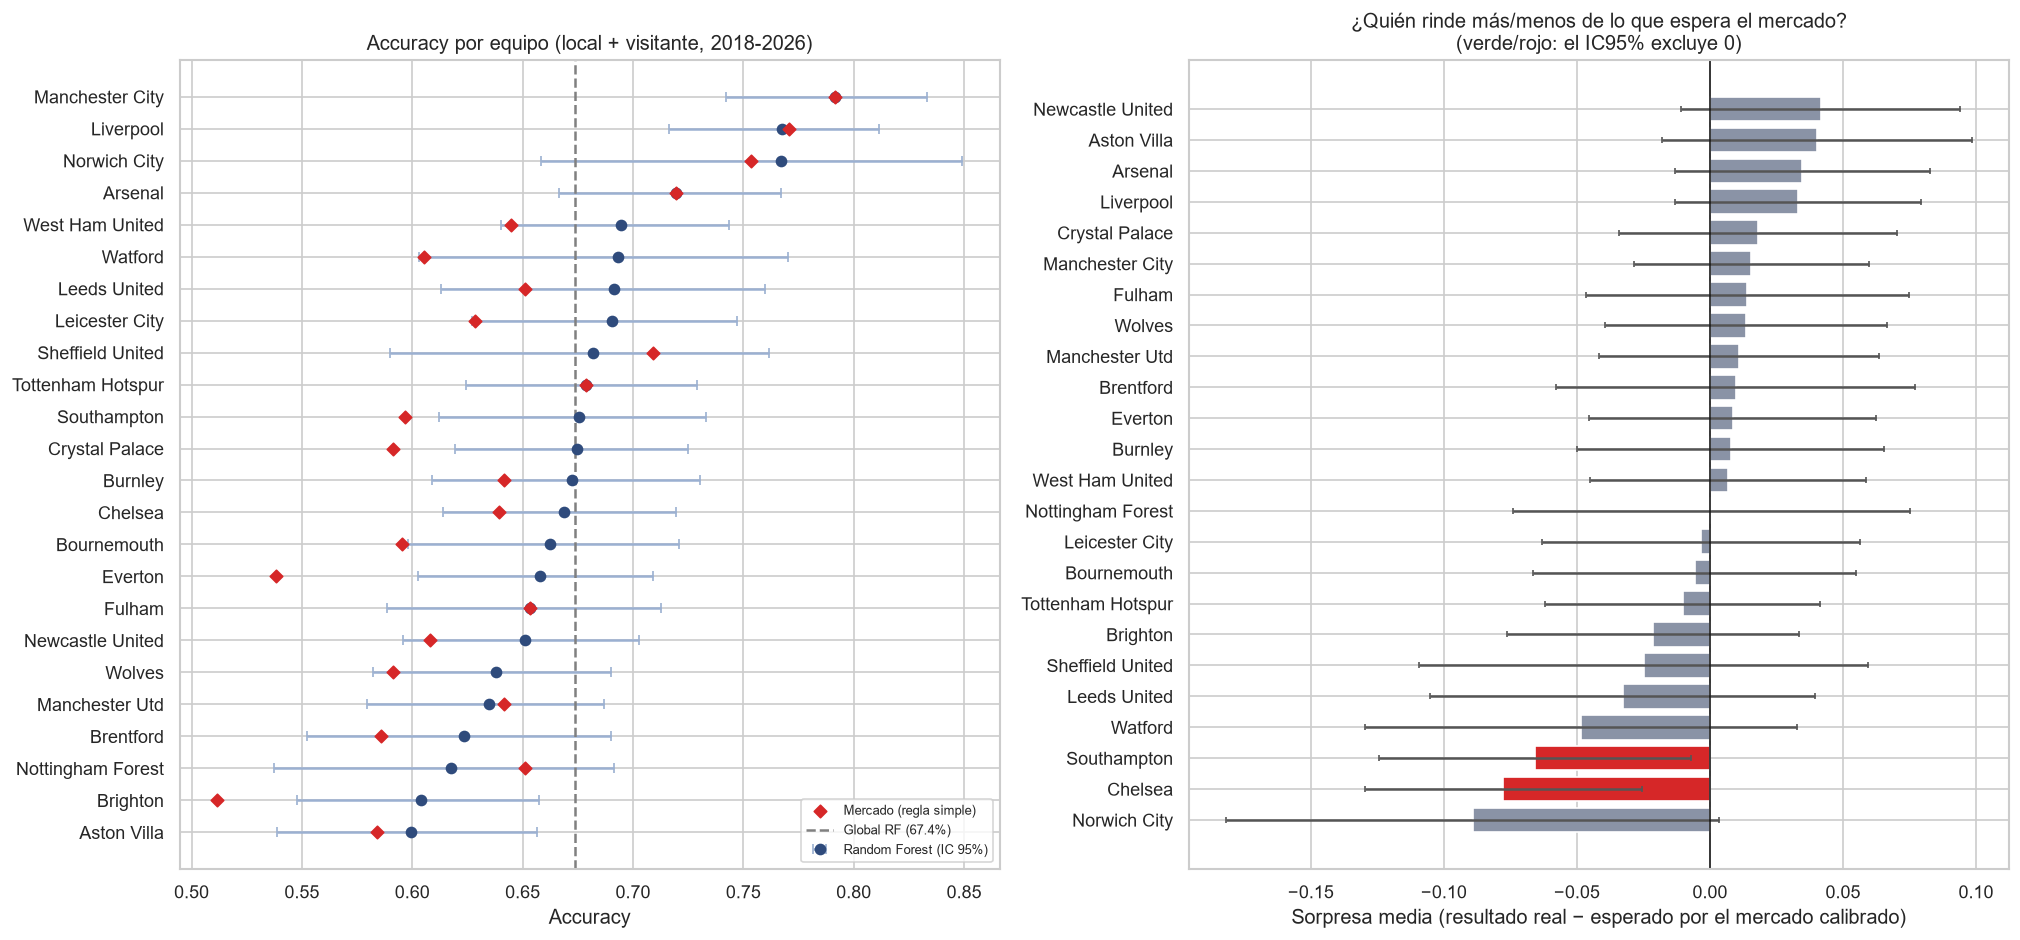
\includegraphics[width=0.95\textwidth]{figuras/analisis_error/por_equipo.png}
\caption[Accuracy de Random Forest por equipo con intervalo de confianza (izquierda) y sorpresa media respecto de las cuotas (derecha)]{Accuracy de Random Forest por equipo con intervalo de confianza (izquierda) y sorpresa media respecto de las cuotas (derecha). Fuente: elaboración propia con datos de FBref y football-data.co.uk.}
\label{fig:equipos}
\end{figure}

\textbf{Equipos con mejor y peor acierto.} Random Forest acierta más con Manchester City (79,1\%; IC 74,2--83,3), Liverpool (76,7\%) y Arsenal (71,9\%), y menos con Aston Villa (59,9\%), Brighton (60,4\%), Nottingham Forest (61,7\%), Brentford (62,4\%) y Manchester United (63,5\%). El rango entre equipos es de 19,2 puntos, pero con unos 280 partidos por equipo el azar por sí solo explica variaciones de $\pm$5,5 puntos. Tras la corrección por comparaciones múltiples, únicamente Manchester City ($q<0{,}001$) y Liverpool ($q=0{,}007$) difieren significativamente del promedio; Aston Villa y Brighton quedan en el límite ($q=0{,}07$). La razón es estructural: los equipos dominantes son favoritos casi siempre y el modelo, al seguir las cuotas, acierta en la mayoría de esos partidos. Los errores más confiados de todo el período también se concentran en ellos: de los 60 mayores, 21 involucran a Liverpool y 17 a Manchester City (por ejemplo, Manchester City 0--2 Wolves en 2019--20, con 0,91 de probabilidad de victoria local).

\textbf{Diferencias entre local y visitante.} El accuracy por equipo como local y como visitante apenas se correlaciona (0,25). Hay equipos que se predicen mejor como visitantes (Fulham, 59,5\% local frente a 71,2\% visitante; Arsenal; Chelsea) y otros como locales (Crystal Palace, 72,8\% frente a 62,0\%; Southampton; Leeds), pero con 100 a 150 partidos por lado estas diferencias son compatibles con el azar.

\textbf{Equipos que rinden distinto de lo esperado.} Solo Chelsea ($-0{,}078$) y Southampton ($-0{,}066$) tienen una sorpresa media cuyo intervalo de confianza excluye el cero, es decir, rindieron menos de lo que las cuotas esperaban. Sin embargo, son 2 de 24 equipos evaluados sin corrección por multiplicidad, por lo que no constituyen evidencia firme de un sesgo del mercado.

\textbf{Dónde se concentran los errores.} Por tipo de resultado, Random Forest acierta el 78,9\% de las victorias visitantes, el 64,4\% de los empates y solo el 60,2\% de las victorias locales; el 53,5\% de sus errores son victorias locales que no anticipó, el 25,1\% empates y el 21,4\% victorias visitantes predichas como locales. Por tipo de partido, el modelo acierta 80,8\% cuando el visitante es muy favorito (probabilidad local $<30\%$) y 76,7\% cuando el local es muy favorito ($>75\%$), pero solo 55,9\% en partidos parejos (45 a 60\%). Además, los errores son en gran parte los del propio mercado: en el 72\% de los 980 errores de Random Forest la regla del mercado también falla, y Random Forest y la regresión sobre cuotas coinciden en el 93\% de los partidos. En conjunto, la dificultad de predecir se explica más por la incertidumbre inherente de los partidos parejos y por los empates que por equipos particulares.

\chapter{DISCUSIÓN Y LIMITACIONES}
\label{sec:discusion}

\section{Comparación con la literatura}
Las cifras de este trabajo no son comparables directamente con las de Vujčić et al.~\cite{vujcic2026supervised} (77,01\%, promedio entre modelos por equipo con otras variables y un único corte temporal) ni con las de Ajulo y Tiamiyu~\cite{ajulo2026ml} (87,14\%, con variables del propio partido). El propio proceso de este proyecto aporta evidencia de por qué esas cifras deben leerse con cautela: con una fuga de información temporal, Gradient Boosting alcanzó 74,65\% y un AUC de 0,804, y al eliminarla las métricas cayeron a 65,8\% y 0,704. Los valores actuales son del mismo orden que los de Chowdary~\cite{chowdary2026dynamic} en la Premier League (67,7\% con 24 temporadas, aunque con una definición de la tarea no necesariamente idéntica) y superan el 63,0\% de Sjöberg~\cite{sjoborg2023football}, que usa tres clases, 219 partidos y una partición aleatoria. Ridall et al.~\cite{ridall2025bayesian} y Baboota y Kaur~\cite{baboota2019predictive} usan RPS sobre tres clases, métrica no comparable con el accuracy binario de este trabajo, pero coinciden en la conclusión central: no es posible superar a las casas de apuestas.

\section{Interpretación de los resultados}
Los resultados convergen en que las cuotas concentran casi toda la información predecible con los datos disponibles: (i) la regresión logística con solo las tres probabilidades implícitas tiene el mejor ROC-AUC y log-loss de todos los modelos y un accuracy equivalente al de los modelos con 28 variables (68,3 a 68,6\% con probabilidades calibradas); (ii) las 27 variables restantes, incluyendo forma, plantel, porteros y enfrentamientos directos, no mejoran la predicción cuando están las cuotas; (iii) sin cuotas, los modelos solo igualan la regla simple del mercado; (iv) la mezcla de modelos y la optimización por calidad de probabilidad no superan a las cuotas solas; y (v) las redes neuronales, incluida la optimizada con Keras Tuner, no mejoran a los modelos más simples. Es coherente con un mercado informacionalmente eficiente. El aporte medible de los modelos respecto de la regla simple del mercado (+3 a +4 puntos) se explica sobre todo por usar las cuotas de forma calibrada, y no por información adicional.

\section{Validación temporal}
La validación de ventana expansiva garantiza que cada fold se evalúe sobre datos futuros respecto del entrenamiento, y la desviación entre folds (alrededor de 1 a 3 puntos de accuracy, mayor en los primeros folds con pocos datos de entrenamiento) cuantifica la variabilidad entre temporadas.

\section{Limitaciones del estudio}
\begin{enumerate}
\item \textbf{Corrección conjunta de dos errores:} los errores de duplicados y de fechas se corrigieron a la vez, por lo que no se puede atribuir la caída de las métricas a cada uno por separado.
\item \textbf{Selección de variables:} RFECV se aplicó sobre el conjunto completo de datos, por lo que la elección de las 28 variables pudo usar información de temporadas posteriores a algunos folds de test. Una selección anidada dentro de cada fold evitaría este sesgo optimista; dado que los modelos finales no mejoran a las cuotas solas, es poco probable que cambie la conclusión.
\item \textbf{Primera temporada:} las variables de plantel de la temporada 2017--2018 (347 partidos) no tienen temporada previa y se imputaron con la mediana de la liga.
\item \textbf{Tarea binaria:} el problema se redujo a victoria local vs. no victoria local, sin distinguir empates ni usar RPS ni pruebas de significancia (por ejemplo McNemar) frente al mercado; con ~370 partidos por temporada, diferencias menores a 1 punto no son concluyentes.
\item \textbf{Red neuronal PyTorch:} el \textit{early stopping} usó el conjunto de test como validación, lo que favorece levemente a este modelo.
\item \textbf{Red Keras Tuner:} el promedio de 10 redes se decidió tras observar la inestabilidad del fold 1 (véase el Capítulo de resultados); las 20 configuraciones por fold son un presupuesto de búsqueda reducido.
\item \textbf{Análisis sin cuotas:} usa hiperparámetros fijos, no optimizados por fold.
\item \textbf{Variables contextuales ausentes:} lesiones, alineaciones, clima, cambios de entrenador y motivación.
\item \textbf{Prueba con datos reales y análisis por equipo:} la prueba usa una sola temporada (377 partidos) con intervalos de $\pm$5 puntos, por lo que no permite concluir diferencias entre los modelos y el mercado; el análisis por equipo dispone de entre 35 y 300 partidos por equipo, implica muchas comparaciones simultáneas y sus errores son en gran parte compartidos con el mercado.
\item \textbf{Ventana temporal:} ocho temporadas pueden no capturar cambios estructurales de largo plazo.
\end{enumerate}

\chapter{CONCLUSIONES}
\label{sec:conclusiones}
Este proyecto muestra que, con datos validados contra fuga de información y validación temporal estricta, es posible predecir si el equipo local gana un partido de la Premier League con un accuracy cercano a 68\% (Random Forest: 68,2\%; ROC-AUC 0,727), 3,9 puntos porcentuales sobre la regla simple del mercado (64,4\%) y superándola en los 7 folds. Sin embargo, ningún modelo supera a una regresión logística entrenada solo con las probabilidades de las cuotas (68,6\% de accuracy con probabilidades calibradas, ROC-AUC 0,736, el mejor de todos), por lo que el objetivo de superar al mercado se cumple únicamente frente a la regla simple. Los objetivos específicos se cumplieron así:
\begin{enumerate}
\item Se construyó y validó un conjunto de datos de ocho temporadas (3.040 partidos, 2.973 para modelado), y el control de calidad detectó y corrigió dos errores que habían inflado los resultados iniciales.
\item Se diseñó un proceso de \textit{feature engineering} con forma reciente, H2H, plantel y porteros, y RFECV redujo 58 candidatas a 28 variables.
\item Se compararon siete algoritmos, incluida una red neuronal optimizada con Keras Tuner, con validación de ventana expansiva; los modelos más simples (regresión logística, Random Forest) rinden igual o mejor que los más complejos.
\item Se evaluó con accuracy, F1, ROC-AUC, Brier y log-loss frente a dos referencias del mercado; sin cuotas, los modelos solo igualan la regla simple, y la mezcla de modelos no mejora a las cuotas solas.
\item El análisis de interpretabilidad (Gini, permutación y SHAP global y por partido) mostró que la probabilidad implícita del mercado domina la predicción y que la mayoría de las variables adicionales no aporta.
\item Una prueba con la temporada 2025--26, no usada en ninguna decisión, dio 61,3\% (Random Forest) y 62,9\% (solo cuotas) frente a 60,5\% de la regla del mercado, sin diferencias significativas; el análisis de error por equipo mostró que el modelo acierta más con los equipos dominantes (Manchester City, 79,1\%; Liverpool, 76,7\%) y menos en partidos parejos y empates, y que el 72\% de sus errores también los comete el mercado.
\item Se documentó el proceso completo en este informe y en el repositorio del proyecto.
\end{enumerate}

Además de los resultados de predicción, un aporte metodológico del trabajo es el control de calidad: los errores de datos, que inflaban el accuracy entre 3 y 10 puntos según el modelo, pasaron inadvertidos hasta que se contrastaron con un validador independiente, lo que subraya la importancia de verificar la ausencia de fuga de información antes de interpretar métricas elevadas.

Como trabajo futuro se propone: (i) realizar la selección de variables dentro de cada fold; (ii) abordar el problema en tres clases (local, empate, visitante) y medirlo con RPS y pruebas de significancia para compararlo directamente con Baboota y Kaur y con Ridall et al.; (iii) modelar la corrección sobre las probabilidades del mercado en lugar de predecir desde cero, con fuerte regularización; (iv) incorporar información contextual (lesiones, suspensiones, cambios de entrenador, descanso entre partidos y ratings de fuerza); (v) explorar modelos de secuencia (LSTM, Transformers); y (vi) evaluar la generalización a otras ligas europeas.

\clearpage
\chapter*{GLOSARIO}
\addcontentsline{toc}{chapter}{GLOSARIO}
\begin{description}\setlength\itemsep{2pt}
\item[Accuracy] Porcentaje de partidos clasificados correctamente.
\item[AUC-ROC] Probabilidad de que el modelo asigne una probabilidad mayor a un partido con victoria local que a uno sin ella; 0,5 equivale al azar y 1 es perfecto.
\item[Brier] Error cuadrático medio de las probabilidades predichas; menor es mejor.
\item[Calibración] Grado en que las probabilidades predichas coinciden con las frecuencias reales (de los partidos con 70\% de probabilidad, ocurre cerca del 70\%).
\item[Cuotas] Valores que ofrece una casa de apuestas por cada resultado; su inverso (1/cuota) es la probabilidad implícita.
\item[Fold] Cada una de las particiones entrenamiento--prueba de la validación; aquí, una temporada de prueba con todas las anteriores como entrenamiento.
\item[Fuga de información] Uso, durante el entrenamiento o al construir variables, de datos que no estarían disponibles al momento de predecir.
\item[Head-to-head (H2H)] Historial de enfrentamientos directos previos entre los dos equipos de un partido.
\item[Intervalo de Wilson] Intervalo de confianza para una proporción, como el accuracy.
\item[Log-loss] Medida de calidad de las probabilidades que penaliza fuertemente los errores cometidos con alta confianza; menor es mejor.
\item[McNemar] Prueba estadística para decidir si dos modelos difieren de forma significativa sobre los mismos partidos.
\item[Regla simple del mercado] Predecir victoria local si la probabilidad implícita del local supera a la del visitante.
\item[RFECV] Eliminación recursiva de variables con validación cruzada, usada para seleccionar variables.
\item[RPS] \textit{Ranked Probability Score}: medida de calidad de probabilidades sobre resultados ordenados (local, empate, visitante).
\item[SHAP] Método que descompone cada predicción en la contribución de cada variable.
\item[Ventana expansiva] Esquema de validación donde el entrenamiento crece con cada fold, usando todo el pasado.
\item[Ventana móvil] Cálculo de una variable con solo los últimos $n$ partidos del equipo (aquí $n=5$).
\end{description}

\clearpage
\addcontentsline{toc}{chapter}{REFERENCIAS BIBLIOGRÁFICAS}
\begin{singlespace}
\bibliographystyle{IEEEtran}
\bibliography{references}
\end{singlespace}

\end{document}
